%%%%%%%%%%%%%%%%%%%%%%%%%%%%%%%%%%%%%%%%%%%%%%%%%%%%%%
% A Beamer template for University of Wollongong     %
% Based on THU beamer theme                          %
% Author: Qiuyu Lu                                   %
% Date: July 2024                                    %
% LPPL Licensed.                                     %
%%%%%%%%%%%%%%%%%%%%%%%%%%%%%%%%%%%%%%%%%%%%%%%%%%%%%%
% Customized for Sharif University of Technology     %
%%%%%%%%%%%%%%%%%%%%%%%%%%%%%%%%%%%%%%%%%%%%%%%%%%%%%%


\documentclass[serif, aspectratio=169]{beamer}
%\documentclass[serif]{beamer}  % for 4:3 ratio
\usepackage[T1]{fontenc} 
\usepackage{fourier} % see "http://faq.ktug.org/wiki/uploads/MathFonts.pdf" for other options
\usepackage{hyperref}
\usepackage{latexsym,amsmath,xcolor,multicol,booktabs,calligra}
\usepackage{graphicx,pstricks,listings,stackengine}
\usepackage{lipsum}

% For writing clean pseudocodes
\usepackage{algorithm, algpseudocode, mathtools, needspace}
% To justify the items
\usepackage{ragged2e}
% To draw diagrams
\usepackage{tikz}
% To include urls
\usepackage{url}
% To make clean tables
\usepackage{color, tabularray}

\author{Ali Sharifi-Zarchi}
\title{Machine Learning (CE 40717)}
\subtitle{Fall 2024}
\institute{
    CE Department \\
    Sharif University of Technology
}
\usepackage{SUTstyle}

% defs
\def\cmd#1{\texttt{\color{red}\footnotesize $\backslash$#1}}
\def\env#1{\texttt{\color{blue}\footnotesize #1}}
\definecolor{deepblue}{rgb}{0,0,0.5}
\definecolor{deepred}{RGB}{153,0,0}
\definecolor{deepgreen}{rgb}{0,0.5,0}
\definecolor{halfgray}{gray}{0.55}
\definecolor{silver}{rgb}{0.752,0.752,0.752}

\lstset{
    basicstyle=\ttfamily\small,
    keywordstyle=\bfseries\color{deepblue},
    emphstyle=\ttfamily\color{deepred},    % Custom highlighting style
    stringstyle=\color{deepgreen},
    numbers=left,
    numberstyle=\small\color{halfgray},
    rulesepcolor=\color{red!20!green!20!blue!20},
    frame=shadowbox,
}

% For writing comments that are aligned to the left side
\makeatletter
\NewDocumentCommand{\LeftComment}{s m}{%
  \Statex \IfBooleanF{#1}{\hspace*{\ALG@thistlm}}\(\triangleright\) #2}
\makeatother
% To manually indent states in algorithmicx
\newcommand{\IndState}{\State\hspace{\algorithmicindent}}
% To make breakable algorithms
\makeatletter
\newenvironment{nofloatalgorithmic}[2][0]
  {
  \par
  \needspace{\dimexpr\baselineskip+6.8pt}
  \noindent
  \hrule height.8pt depth0pt \kern2pt
  \refstepcounter{algorithm}
  \addcontentsline{loa}{algorithm}{\numberline{\thealgorithm}#2}
  \noindent\textbf{\fname@algorithm~\thealgorithm} #2\par
  \kern2pt\hrule\kern2pt
  \begin{algorithmic}[#1]
  }
  {
  \end{algorithmic}
  \nobreak\kern2pt\hrule\relax
  }
\makeatother
% To make vertical arrow
\newcommand\vertarrowbox[3][6ex]{%
  \begin{array}[t]{@{}c@{}} #2 \\
  \left\uparrow\vcenter{\hrule height #1}\right.\kern-\nulldelimiterspace\\
  \makebox[0pt]{\scriptsize#3}
  \end{array}%
}
% Clean argmin
\DeclareMathOperator*{\argmin}{arg\,min}

\begin{document}

\begin{frame}
    \titlepage
    \vspace*{-0.6cm}
    \begin{figure}[htpb]
        \begin{center}
            
\includegraphics[keepaspectratio, scale=0.25]{pic/sharif-main-logo.png}
        \end{center}
    \end{figure}
\end{frame}

\begin{frame}    
    \tableofcontents[sectionstyle=show,
    subsectionstyle=show/shaded/hide,
    subsubsectionstyle=show/shaded/hide]
\end{frame}

\section{Introduction}

\subsection{Condorcet's jury theorem}

\begin{frame}{Condorcet's jury theorem}
    \minipage{0.54\textwidth}
    \begin{itemize}
        \itemsep1em
        \justifying
        \item $\boldsymbol{N}$ voters wish to reach a decision by \textbf{majority vote}.
        \item Each voter has an independent probability $\boldsymbol{p}$ of voting for the correct decision.
        \item Let $\boldsymbol{M}$ be the probability of the majority voting for the correct decision.
        \item \textcolor{deepred}{If $\boldsymbol{p > 0.5}$ and $\boldsymbol{N \to \infty}$, then $\boldsymbol{M \to 1}$}
        \begin{itemize}
            \item How?
        \end{itemize}
    \end{itemize}
    \endminipage
    \hfill
    \minipage{0.42\linewidth}
    \begin{figure}[!htb]
        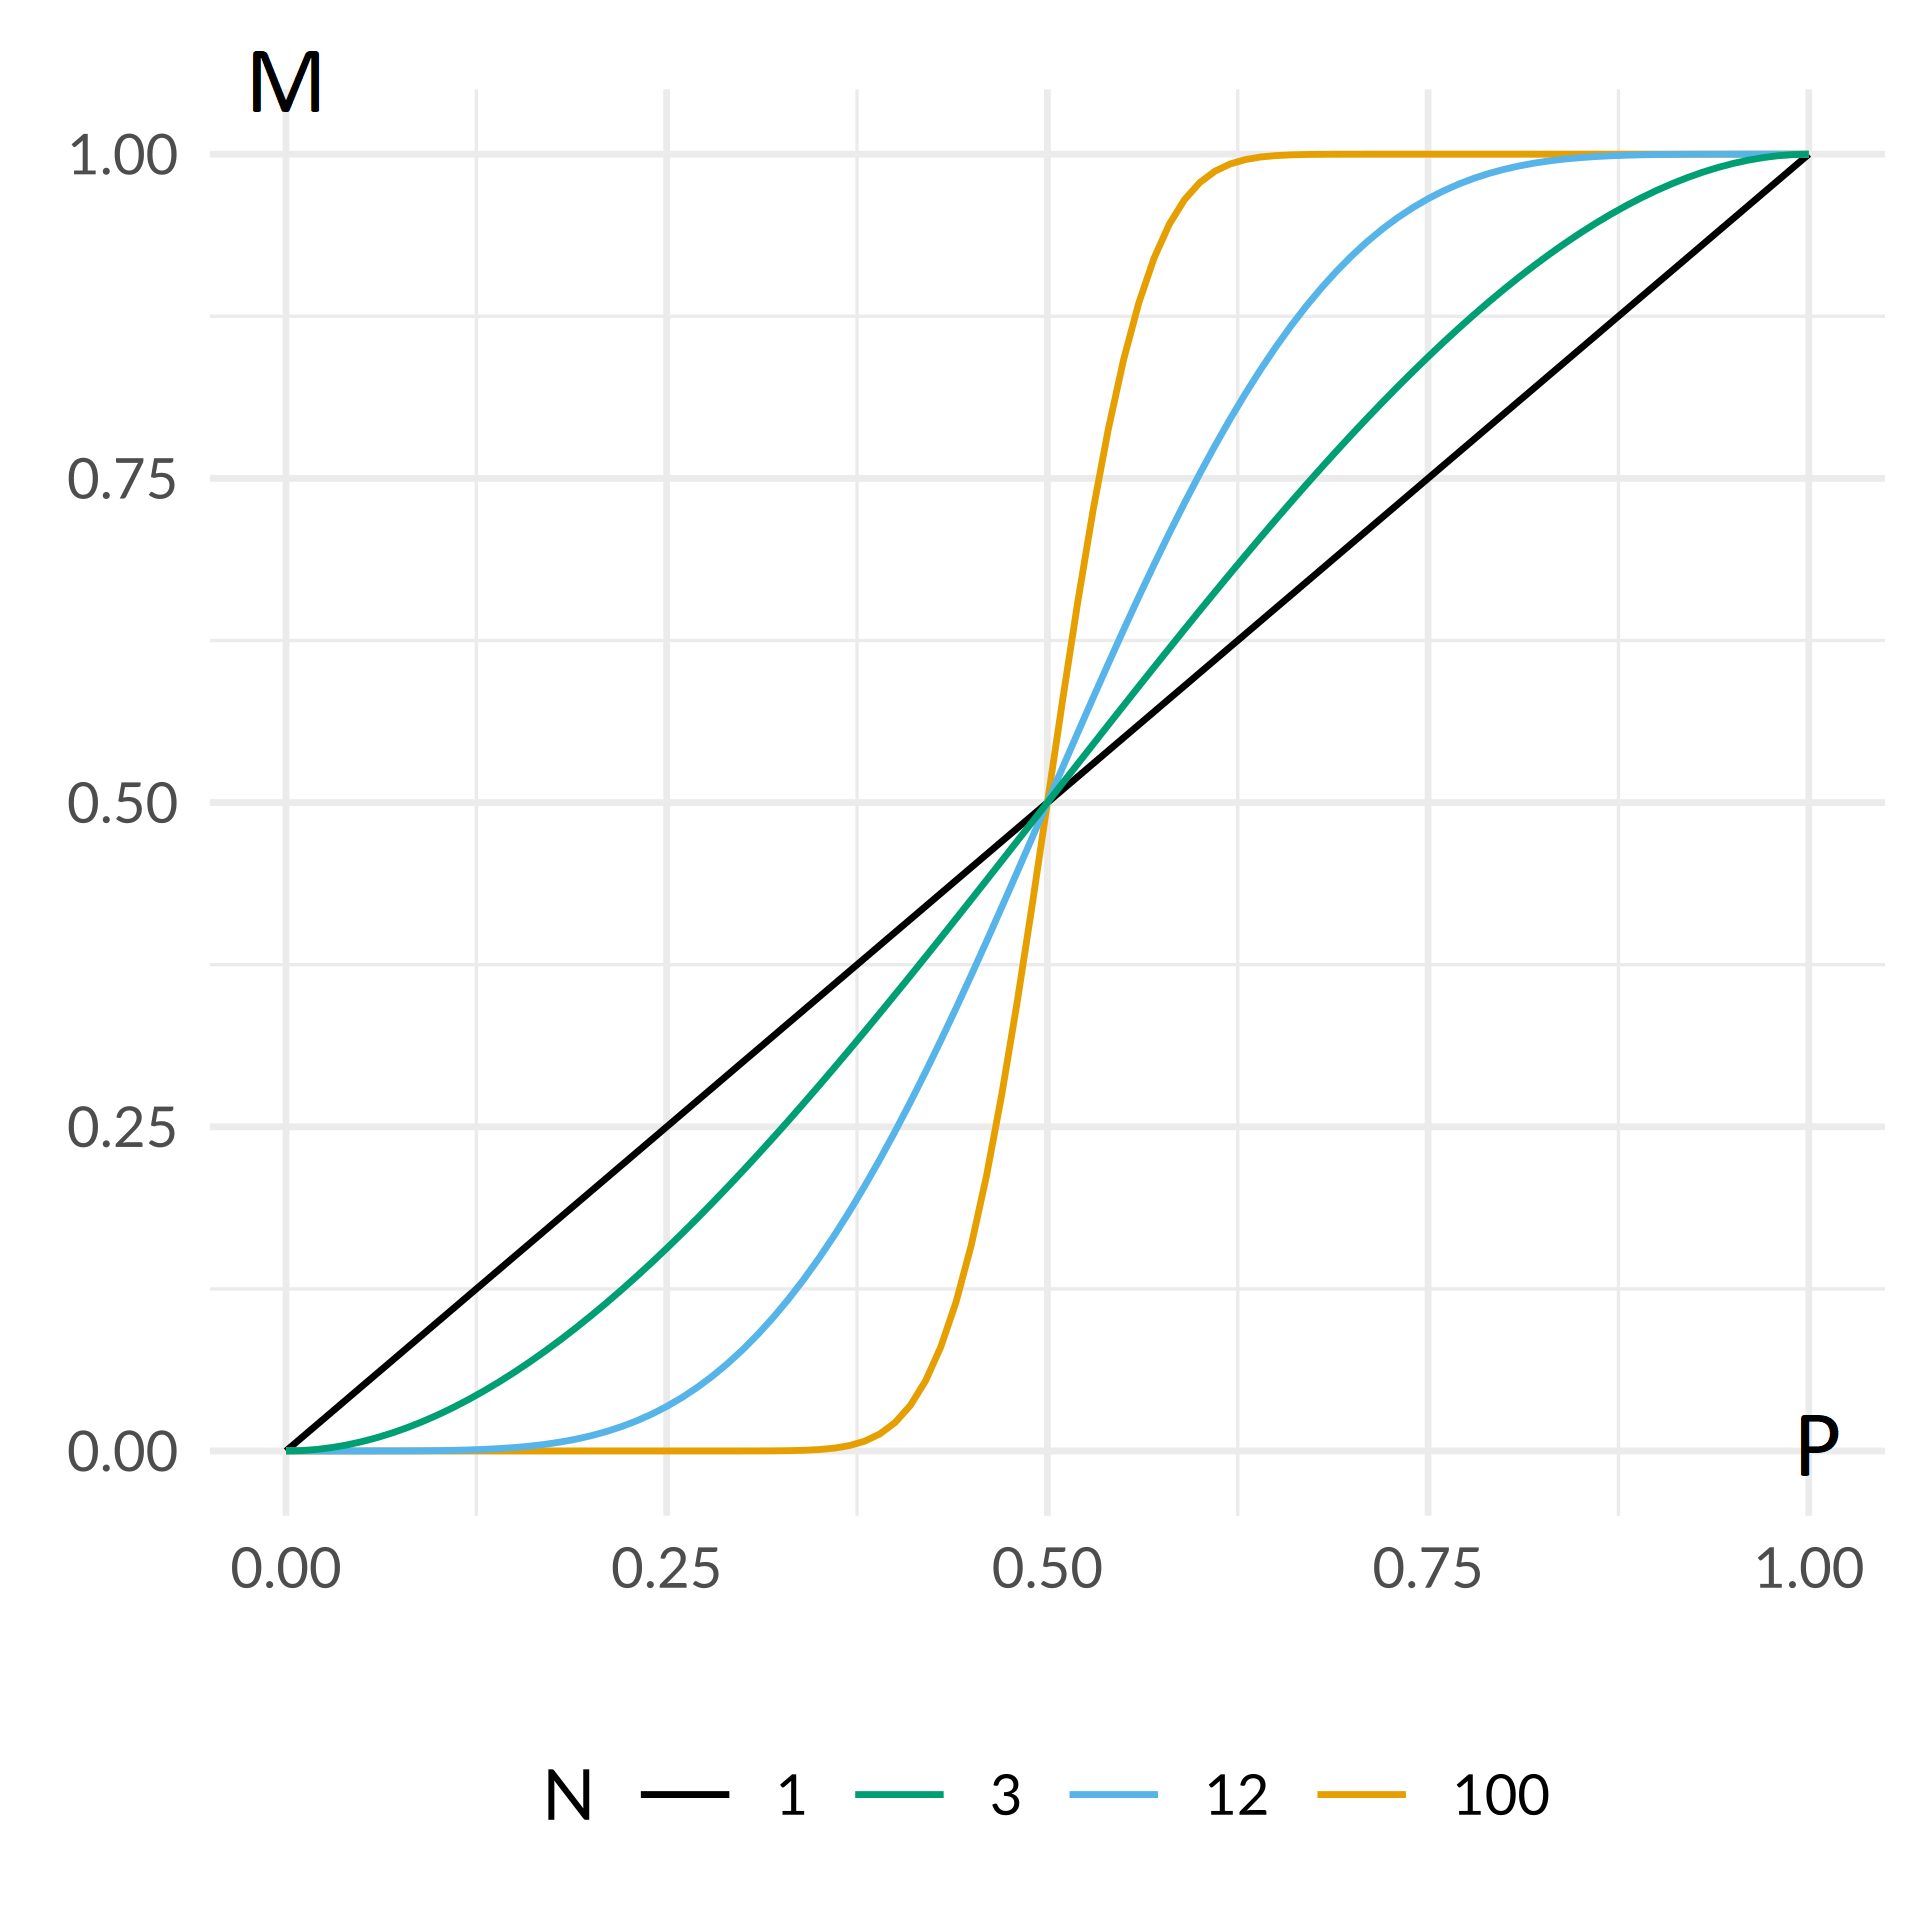
\includegraphics[width=\linewidth]{pic/condorcets.png}
        {\scriptsize Adopted from \href{https://en.wikipedia.org/wiki/Condorcet\%27s_jury_theorem}{Wikipedia}}
    \end{figure}
    \endminipage
\end{frame}

\subsection{Ensemble learning}

\begin{frame}{Strong vs. weak Learners}
    \begin{itemize}
        \itemsep1em
        \justifying
        \item \textbf{Strong learner:} we seek to produce one classifier for which the classification error can be made arbitrarily small.
        \begin{itemize}
            \item So far we were looking for such methods.
        \end{itemize}
        \item \textbf{Weak learner:} a classifier which is just better than random guessing (for now this will be our only expectation).
    \end{itemize}
\end{frame}

\begin{frame}{Basic idea}
    \minipage{0.52\textwidth}
    \begin{itemize}
        \itemsep1em
        \justifying
        \item Certain \textbf{weak learners} do well in modeling one aspect of the data, while others do well in modeling another.
        \item Learn several simple models and \textbf{combine} their outputs to produce the final decision.
        \item A \textbf{composite prediction} where the final accuracy is \textbf{better} than the accuracy of \textbf{individual models}.
    \end{itemize}
    \endminipage \hfill
    \minipage{0.42\textwidth}
    \begin{figure}[!htb]
        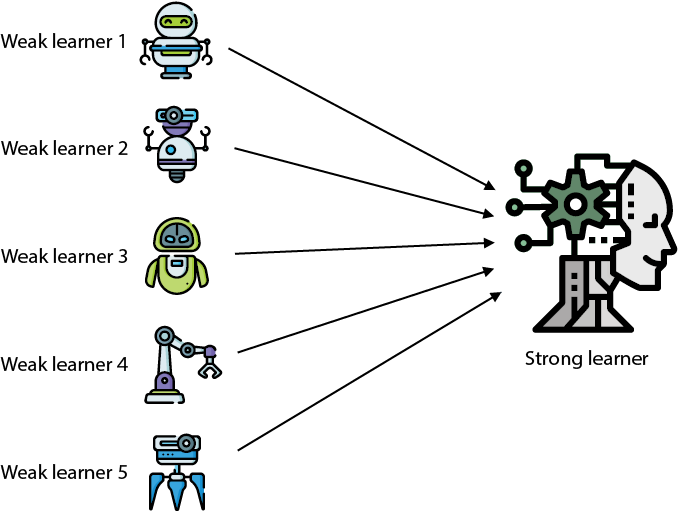
\includegraphics[width=\linewidth]{pic/learners.png}
        {\scriptsize Adopted from [4]}
    \end{figure}
    \endminipage
\end{frame}

\subsection{Ensemble Methods}

\begin{frame}{Ensemble Methods}
    \minipage{0.44\textwidth}
    \tikzset{every picture/.style={line width=1pt}} 
    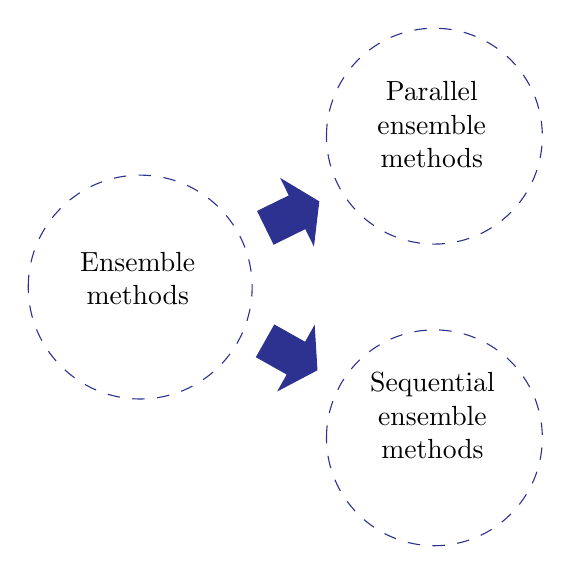
\begin{tikzpicture}[x=0.75pt,y=0.75pt,yscale=-1,xscale=1]
    %Shape: Circle [id:dp3069754614355109] 
    \draw  [color={rgb, 255:red, 45; green, 50; blue, 145 }  ,draw opacity=1 ][dash pattern={on 4.5pt off 4.5pt}] (52.31,155.38) .. controls (52.31,125.59) and (76.46,101.44) .. (106.25,101.44) .. controls (136.04,101.44) and (160.19,125.59) .. (160.19,155.38) .. controls (160.19,185.17) and (136.04,209.31) .. (106.25,209.31) .. controls (76.46,209.31) and (52.31,185.17) .. (52.31,155.38) -- cycle ;
    %Shape: Circle [id:dp039894474724192275] 
    \draw  [color={rgb, 255:red, 45; green, 50; blue, 145 }  ,draw opacity=1 ][dash pattern={on 4.5pt off 4.5pt}] (196,82.67) .. controls (196,53.95) and (219.28,30.67) .. (248,30.67) .. controls (276.72,30.67) and (300,53.95) .. (300,82.67) .. controls (300,111.39) and (276.72,134.67) .. (248,134.67) .. controls (219.28,134.67) and (196,111.39) .. (196,82.67) -- cycle ;
    %Shape: Circle [id:dp8826979851888883] 
    \draw  [color={rgb, 255:red, 45; green, 50; blue, 145 }  ,draw opacity=1 ][dash pattern={on 4.5pt off 4.5pt}] (196,228) .. controls (196,199.28) and (219.28,176) .. (248,176) .. controls (276.72,176) and (300,199.28) .. (300,228) .. controls (300,256.72) and (276.72,280) .. (248,280) .. controls (219.28,280) and (196,256.72) .. (196,228) -- cycle ;
    %Right Arrow [id:dp6293349565535766] 
    \draw  [color={rgb, 255:red, 45; green, 50; blue, 145 }  ,draw opacity=1 ][fill={rgb, 255:red, 45; green, 50; blue, 145 }  ,fill opacity=1 ] (162.91,118.84) -- (178.2,111.34) -- (174.33,103.46) -- (192.26,114.23) -- (189.81,135) -- (185.94,127.11) -- (170.65,134.62) -- cycle ;
    %Right Arrow [id:dp33784620906458995] 
    \draw  [color={rgb, 255:red, 45; green, 50; blue, 145 }  ,draw opacity=1 ][fill={rgb, 255:red, 45; green, 50; blue, 145 }  ,fill opacity=1 ] (170.96,173.74) -- (185.8,182.09) -- (190.11,174.43) -- (191.39,195.31) -- (172.88,205.06) -- (177.18,197.4) -- (162.34,189.06) -- cycle ;
    % Text Node
    \draw (71.75,137.38) node [anchor=north west][inner sep=0.75pt]   [align=left] {\begin{minipage}[lt]{48.08pt}\setlength\topsep{0pt}
    \begin{center}
    Ensemble\\methods
    \end{center}
    \end{minipage}};
    % Text Node
    \draw (211.5,55.17) node [anchor=north west][inner sep=0.75pt]   [align=left] {\begin{minipage}[lt]{50.94pt}\setlength\topsep{0pt}
    \begin{center}
    Parallel\\ensemble\\methods
    \end{center}
    \end{minipage}};
    % Text Node
    \draw (214.5,195.33) node [anchor=north west][inner sep=0.75pt]   [align=left] {\begin{minipage}[lt]{46.95pt}\setlength\topsep{0pt}
    \begin{center}
    Sequential\\ensemble\\methods
    \end{center}
    \end{minipage}};
    \end{tikzpicture}
    \endminipage
    \hfill
    \minipage{0.54\textwidth}
    \begin{itemize}
        \itemsep1em
        \justifying
        \item Weak learners are generated in \textbf{parallel}.
        \item Basic motivation is to use \textbf{independence} between the learners.
        \vspace{2cm}
        \item Weak learners are generated \textbf{consecutively}.
        \item Basic motivation is to use \textbf{dependence} between the base learners.
    \end{itemize}
    \endminipage
\end{frame}

\begin{frame}{What we talk about}
    \begin{itemize}
        \itemsep1em
        \justifying
        \item Weak or simple learners
        \begin{itemize}
            \itemsep0.25em
            \item \textbf{Low variance}: they don't usually overfit
            \item \textbf{High bias}: they can't learn complex functions
        \end{itemize}
        \item \textbf{Bagging} (parallel): To decrease the variance
        \begin{itemize}
            \item Random Forest
        \end{itemize}
        \item \textbf{Boosting} (sequential): To decrease the bias (enhance their capabilities)
        \begin{itemize}
            \item AdaBoost
        \end{itemize}
    \end{itemize}
\end{frame}

\section{Bagging}

\subsection{Basic idea \& algorithm}

\begin{frame}{Basic idea}
    \begin{itemize}
        \itemsep1em
        \justifying
        \item \textbf{Bagging} = \textbf{B}ootstrap \textbf{agg}regat\textbf{ing}
        \item It uses \textbf{bootstrap resampling} to generate different training datasets from the original training dataset.
        \begin{itemize}
            \item Samples training data uniformly at random with replacement.
        \end{itemize}
        \item On the training datasets, it trains different weak learners.
        \item During testing, it \textbf{aggregates} the weak learners by uniform averaging or majority voting.
        \begin{itemize}
            \item Works best with unstable models (high variance models). Why?
        \end{itemize}
    \end{itemize}
\end{frame}

\begin{frame}{Basic idea, Cont.}
    \begin{center}
    \minipage{0.8\textwidth}
    \begin{figure}[bh]
        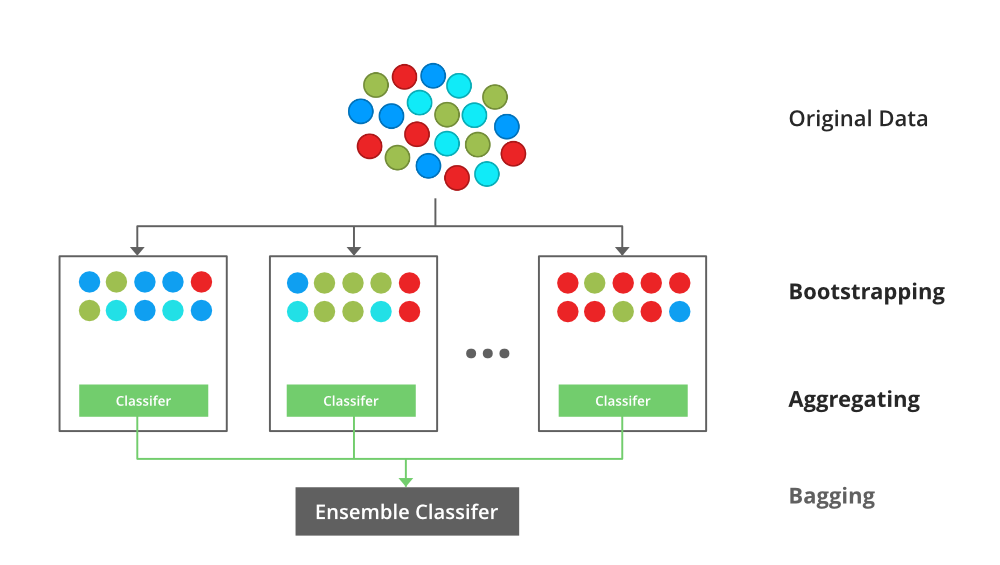
\includegraphics[width=\textwidth]{pic/bagging.png}
        {\scriptsize Adopted from \href{https://www.geeksforgeeks.org/bagging-vs-boosting-in-machine-learning/}{GeeksForGeeks}}
    \end{figure}
    \endminipage
    \end{center}
\end{frame}

\begin{frame}{Algorithm}
    \begin{algorithm}[H]
    \caption{Bagging}\label{alg:Bagging}
    \begin{algorithmic}[1]
        \State \textbf{Input:} $M$ (required ensemble size), $D = \{(\boldsymbol{x}^{(1)}, y^{(1)}), \dots, (\boldsymbol{x}^{(N)}, y^{(N)})\}$ (training set)
    
        \For{$t = 1$ to $M$}
            \State Build a dataset $D_t$ by sampling $N$ items randomly with replacement from $D$
            \LeftComment{\textit{Bootstrap resampling: like rolling N-face dice N times}}
            \State Train a model $h_t$ using $D_t$ and add it to the ensemble
        \EndFor
    
        \State $H(x) = \text{sign}\left(\sum_{t=1}^M h_t(\boldsymbol{x})\right)$
        \LeftComment{\textit{Aggregate models by voting for classification or by averaging for regression}}
    \end{algorithmic}
    \end{algorithm}
\end{frame}

\subsection{Decision tree (quick review)}

\begin{frame}{Structure}
    \minipage{0.49\textwidth}
    \begin{itemize}
        \itemsep1em
        \justifying
        \item \textbf{Terminal nodes} (leaves) represent target variable.
        \item Each \textbf{internal node} denotes a test on an attribute.
    \end{itemize}
    \endminipage
    \hfill
    \minipage{0.44\textwidth}
    \begin{figure}[!htb]
        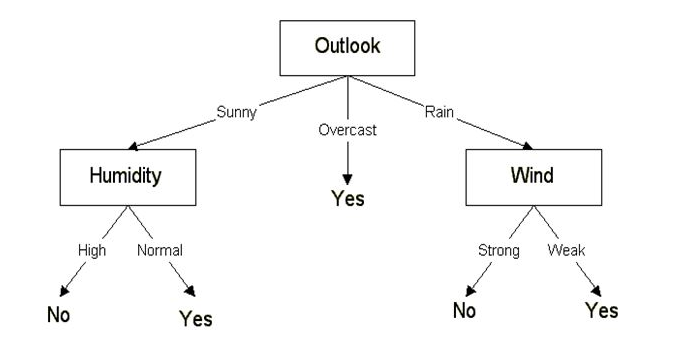
\includegraphics[width=\linewidth]{pic/dt_e.png} \\
        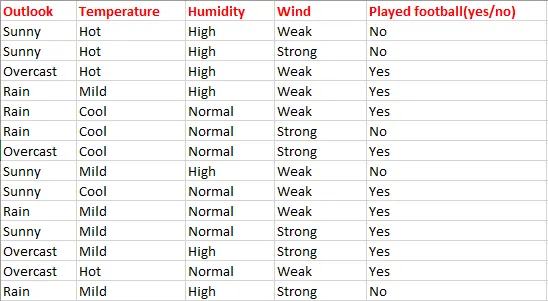
\includegraphics[width=0.85\linewidth]{pic/dt_edataset.png}
        {\scriptsize Adopted from \href{https://medium.datadriveninvestor.com/decision-tree-algorithm-with-hands-on-example-e6c2afb40d38}{Medium}}
    \end{figure}
    \endminipage
\end{frame}

\begin{frame}{Learning}
    \begin{itemize}
        \itemsep1em
        \justifying
        \item Learning an optimal decision tree is \textbf{NP-Complete}.
        \begin{itemize}
            \itemsep0.25em
            \item Instead, we use a \textbf{greedy search} based on a heuristic.
            \item We can't guarantee to return the globally-optimal decision tree.
        \end{itemize}
        \item The most common strategy for DT learning is a greedy top-down approach.
        \item Tree is constructed by splitting samples into subsets based on an \textbf{attribute value test} in a recursive manner.
        \item[] \begin{center}
            Adopted from G.E. Naumov, "NP-completeness of problems of construction of optimal decision trees", 1991
        \end{center}
    \end{itemize}
\end{frame}

\begin{frame}{Algorithm}
    \begin{algorithm}[H]
    \caption{Constructing DT}\label{alg:DT}
    \begin{algorithmic}[1]
    \Procedure{FindTree}{$S$, $A$} \Comment{Input: $S$ (samples), $A$ (attributes)}
        \If {$A$ is empty \textbf{or} all labels in $S$ are the same}
            \State \textbf{status} $\gets$ leaf
            \State \textbf{class} $\gets$ most common class in $S$
        \Else
            \State \textbf{status} $\gets$ internal
            \State $a \gets$ \textcolor{deepred}{bestAttribute($S$, $A$)} \Comment{The attribute value test}
            \State LeftNode $\gets$ FindTree($S(a=1)$, $A - \{a\}$)
            \State RightNode $\gets$ FindTree($S(a=0)$, $A - \{a\}$)
        \EndIf
    \EndProcedure
    \end{algorithmic}
    \end{algorithm}
\end{frame}

\begin{frame}{Which attribute is the best?}
    \minipage{0.54\textwidth}
    \begin{itemize}
        \itemsep1em
        \justifying
        \item \textbf{Entropy} measures the uncertainty in a specific distribution.
        \item[] \begin{center}
            $H(X) = -\displaystyle\sum_{\boldsymbol{x}_i \in \boldsymbol{x}} P(\boldsymbol{x}_i)\log P(\boldsymbol{x}_i)$
        \end{center}
        \item \textbf{Information Gain (IG)}
        \item[] \begin{center}
            $\text{Gain}(S, A) = H_S(Y) - \displaystyle\sum_{v \in \text{Values}(A)} \dfrac{\vert S_v\vert}{\vert S\vert}H_{S_V}(Y)$
        \end{center}
    \end{itemize}
    \begin{itemize}
        \itemsep0.25em
        \justifying
        \item[] $A$: variable used to split samples
        \item[] $Y$: target variable
        \item[] $S$: samples, \qquad $S_v$: subset of $S$ where $A = v$
        \item[] $H_S(Y)$: entropy of $Y$ over $S$
    \end{itemize}
    \endminipage
    \hfill
    \minipage{0.34\textwidth}
    \begin{figure}[!htb]
        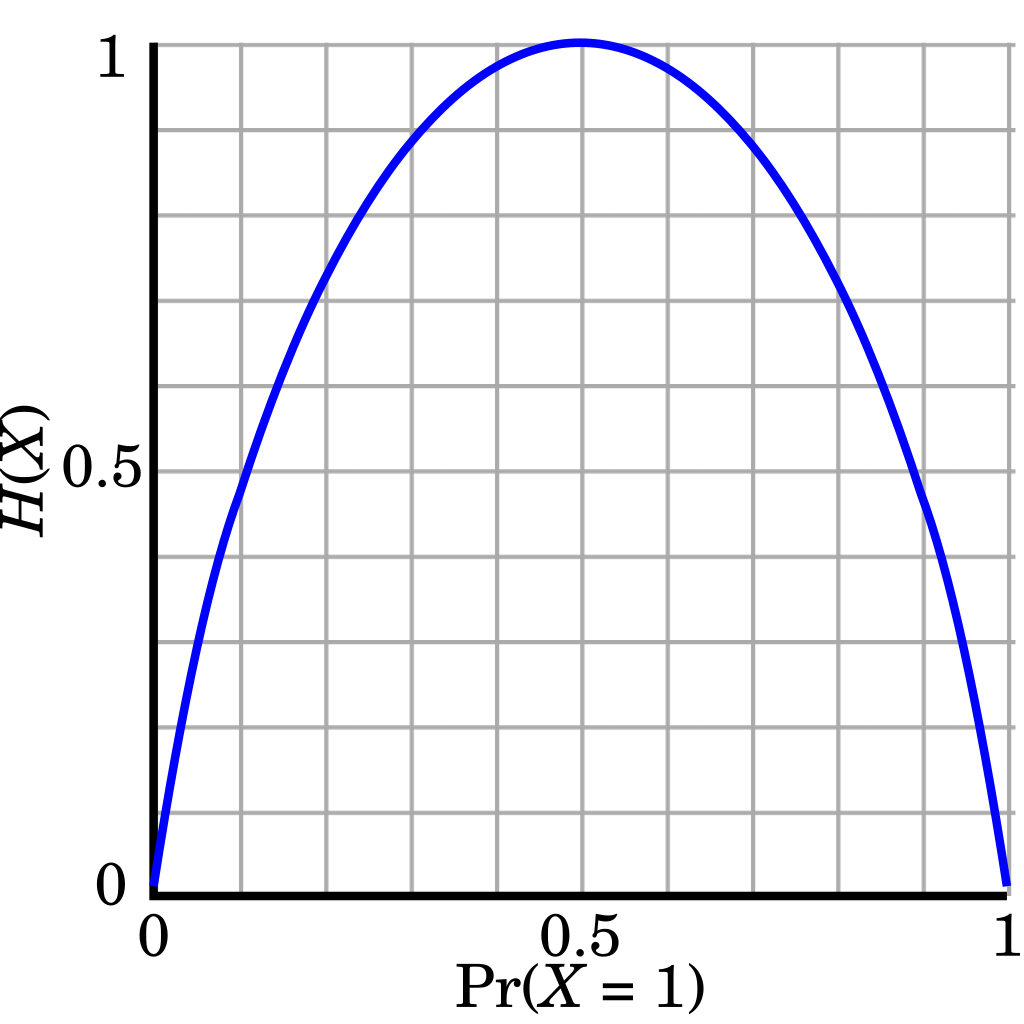
\includegraphics[width=\linewidth]{pic/entropy.png}
        {\scriptsize Adopted from \href{https://en.wikipedia.org/wiki/Binary_entropy_function}{Wikipedia}}
    \end{figure}
    \endminipage
\end{frame}

\begin{frame}{Example}
    \begin{center}
    \minipage{0.66\textwidth}
    \begin{figure}[bh]
        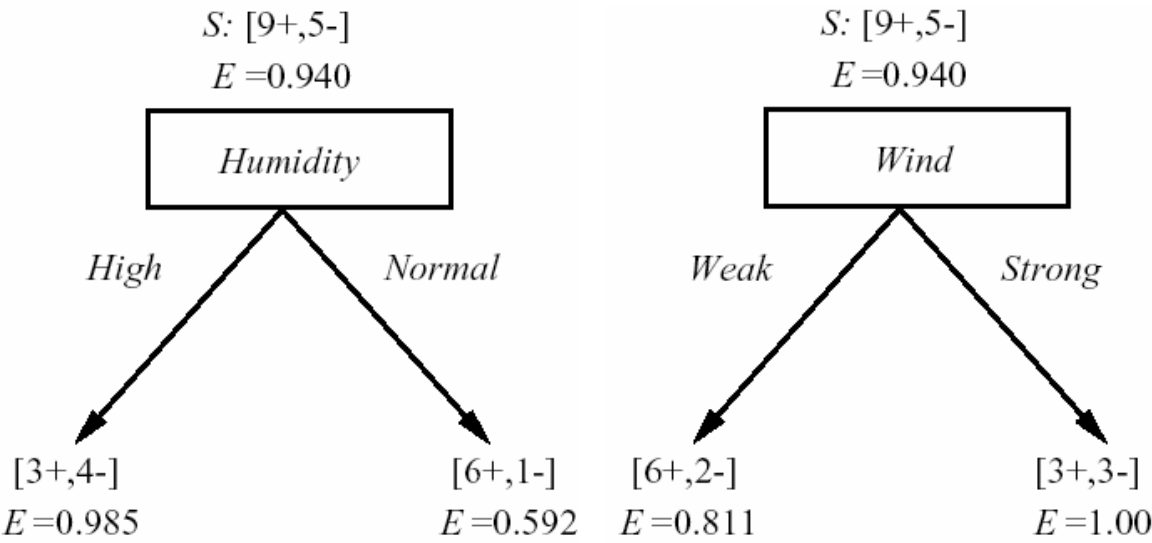
\includegraphics[width=\textwidth]{pic/informationgain.png}
        {\scriptsize Adopted from [5]}
    \end{figure}
    \endminipage
    \end{center}

    \begin{itemize}
    \itemsep1em
    \justifying
    \item[] $\text{Gain}(S, Humidity) = 0.940 - (7/14) 0.985 - (7/14) 0.592 = 0.151$
    \item[] $\text{Gain}(S, Wind) = 0.940 - (8/14) 0.811 - (6/14) 1.0 = 0.48$
    \end{itemize}
\end{frame}

\subsection{Random Forest}

\begin{frame}{Bagging on decision trees?}
    \minipage{0.29\textwidth}
    Why decision trees?
    \begin{itemize}
        \itemsep0.25em
        \justifying
        \item Interpretable
        \item Robust to outliers
        \item \textbf{Low bias}
        \item \textbf{High variance}
    \end{itemize}
    \endminipage
    \hfill
    \minipage{0.65\textwidth}
    \begin{figure}[!htb]
        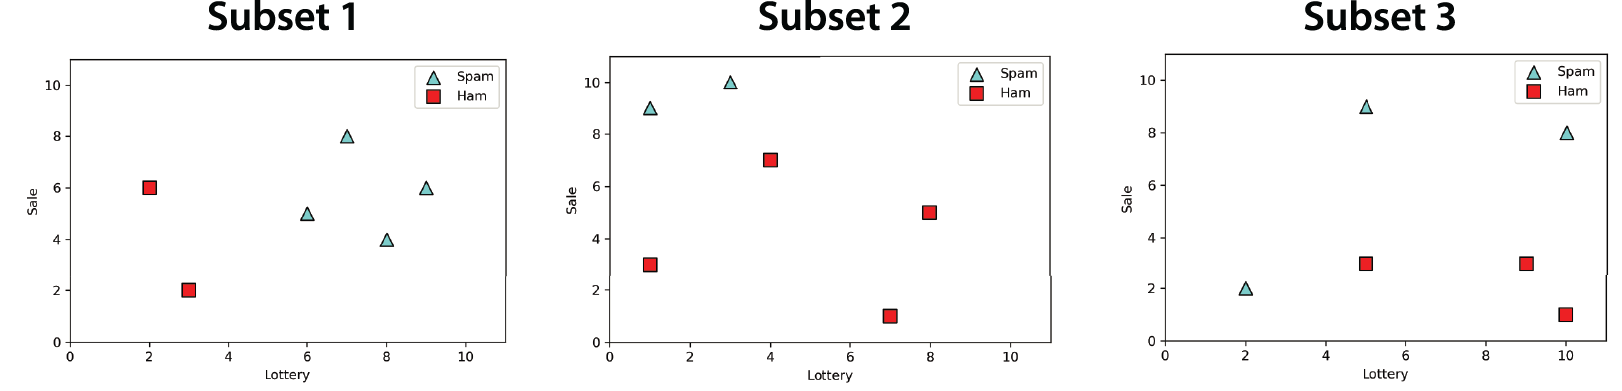
\includegraphics[width=\linewidth]{pic/dt_plot.png} \\ \medskip
        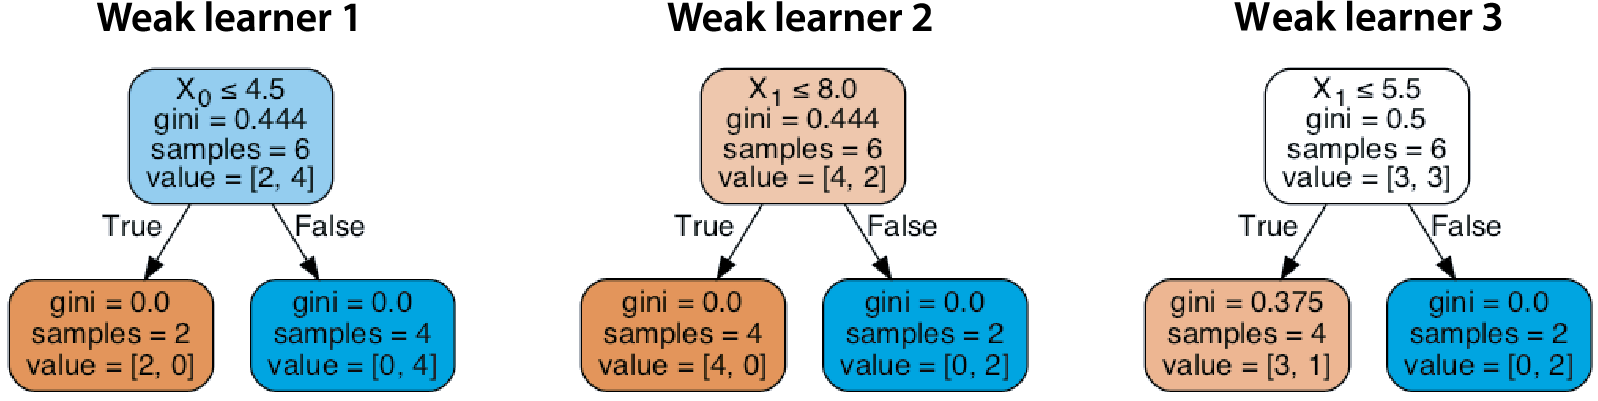
\includegraphics[width=\linewidth]{pic/dt_tree.png}
        {\scriptsize Adopted from [4]}
    \end{figure}
    \endminipage
\end{frame}

\begin{frame}{Perfect candidates}
    \begin{itemize}
        \itemsep1em
        \justifying
        \item Why are \textbf{DTs} good candidates for ensembles?
        \begin{itemize}
            \itemsep0.25em
            \item Consider averaging many (nearly) \textbf{unbiased} tree estimators.
            \item Bias remains similar, but \textbf{variance is reduced}.
        \end{itemize}
        \item Remember Bagging?
        \begin{itemize}
            \item Train many trees on bootstrapped data, then aggregate (average/majority) the outputs.
        \end{itemize}
    \end{itemize}
\end{frame}

\begin{frame}{Algorithm}
    \begin{algorithm}[H]
    \caption{Random Forest}\label{alg:RF}
    \begin{algorithmic}[1]
        \State \textbf{Input:} $T$ (number of trees), $m$ (number of variables used to split each node)
        
        \For{$t = 1$ to $T$}
            \State Draw a bootstrap dataset
            \State \textcolor{deepred}{Select $\boldsymbol{m}$ features randomly out of $\boldsymbol{d}$ features as candidates for splitting}
            \State Learn a tree on this dataset
        \EndFor
        
        \State \textbf{Output:} \Comment{\textit{Usually: $m \leq \sqrt{d}$}}
        \IndState Regression: average of the outputs
        \IndState Classification: majority voting
    \end{algorithmic}
    \end{algorithm}
\end{frame}

\begin{frame}{Example}
    \begin{center}
    \minipage{0.69\textwidth}
    \begin{figure}[bh]
        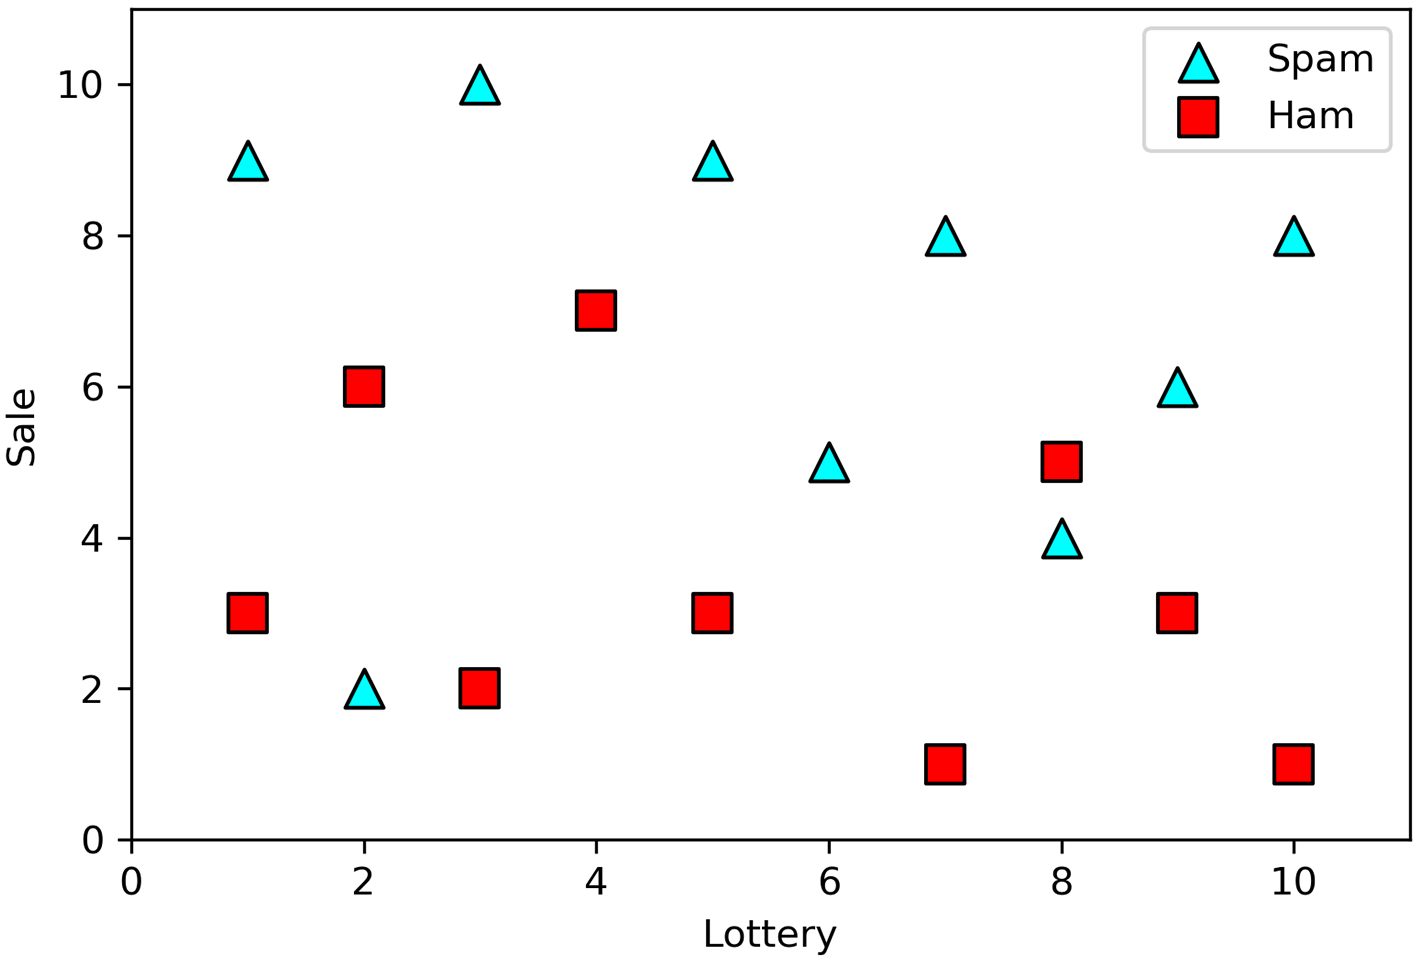
\includegraphics[width=\textwidth]{pic/rf_e1.png}
        {\scriptsize Adopted from [4]}
    \end{figure}
    \endminipage
    \end{center}
\end{frame}

\begin{frame}{Example, Cont.}
    \begin{center}
    \minipage{0.76\textwidth}
    \begin{figure}[!htb]
        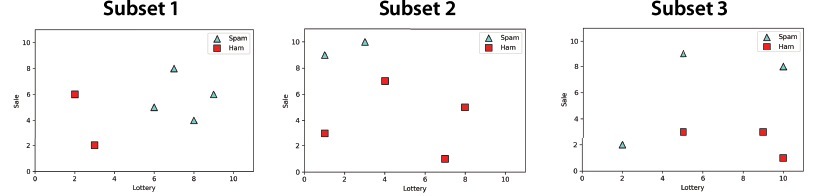
\includegraphics[width=\linewidth]{pic/rf_e2.png} \\
        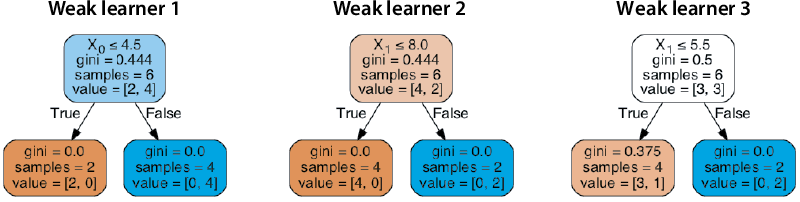
\includegraphics[width=0.85\linewidth]{pic/rf_e3.png} \\
        {\scriptsize Adopted from [4]}
    \end{figure}
    \endminipage
    \end{center}
\end{frame}

\begin{frame}{Example, Cont.}
    \begin{center}
    \minipage{0.76\textwidth}
    \begin{figure}[bh]
        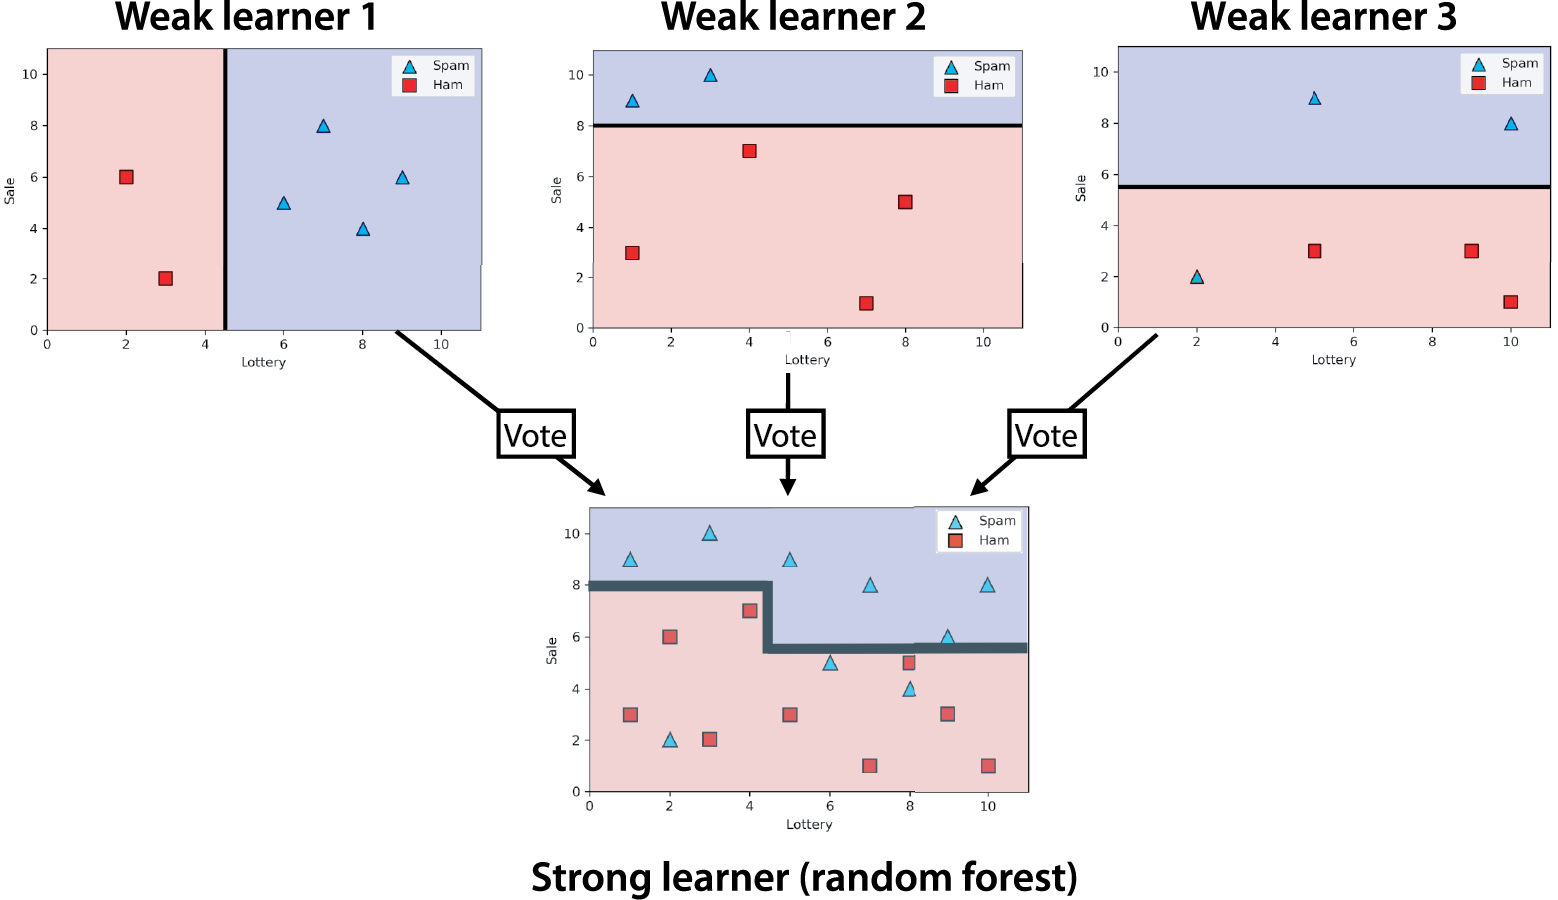
\includegraphics[width=\textwidth]{pic/rf_e4.png}
        {\scriptsize Adopted from [4]}
    \end{figure}
    \endminipage
    \end{center}
\end{frame}

\section{Boosting}

\subsection{Motivation \& basic idea}

\begin{frame}{Problems with bagging}
    \begin{itemize}
        \itemsep1em
        \justifying
        \item Bagging created a diversity of \textbf{weak learners} by creating random datasets.
        \begin{itemize}
            \item Examples: Decision stumps (shallow decision trees), Logistic regression, \dots
        \end{itemize}
        \item Did we have full control over the usefulness of the weak learners?
        \begin{itemize}
            \item The \textbf{diversity} or \textbf{complementarity} of the weak learners is not controlled in any way, it is left to chance and to the instability (variance) of the models.
        \end{itemize}
    \end{itemize}
\end{frame}

\begin{frame}{Basic idea}
    \begin{itemize}
        \itemsep1em
        \justifying
        \item We would expect a better performance if the weak learners also \textbf{complemented} each other.
        \begin{itemize}
            \itemsep0.25em
            \item They would have "expertise" on different subsets of the dataset.
            \item So they would work better on different subsets.
        \end{itemize}
        \item The basic idea of boosting is to generate a \textbf{series} of weak learners which complement each other.
        \begin{itemize}
            \item For this, we will force each learner to focus on \textbf{the mistakes of the previous learner}.
        \end{itemize}
    \end{itemize}
\end{frame}

\begin{frame}{Basic idea, Cont.}
    \begin{center}
    \minipage{0.75\textwidth}
    \begin{figure}[bh]
        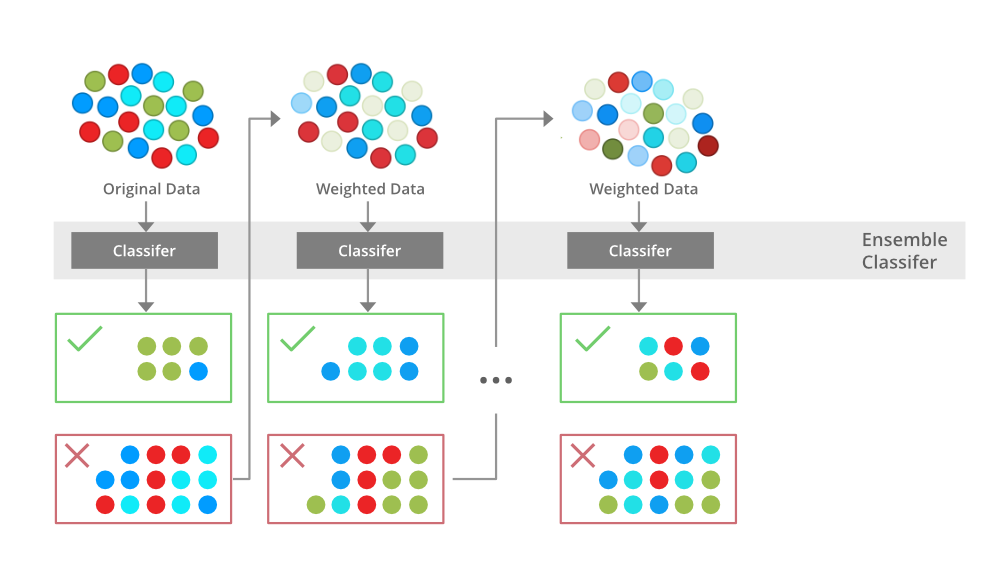
\includegraphics[width=\textwidth]{pic/boosting.png}
        {\scriptsize Adopted from \href{https://www.geeksforgeeks.org/bagging-vs-boosting-in-machine-learning/}{GeeksForGeeks}}
    \end{figure}
    \endminipage
    \end{center}
\end{frame}

\subsection{Algorithm}

\begin{frame}{Algorithm}
    \begin{itemize}
        \itemsep1em
        \justifying
        \item Try to combine many simple \textbf{weak} learners (in sequence) to find a single \textbf{strong} learner (For simplicity, suppose that we have a classification problem from now on).
        \begin{itemize}
            \itemsep0.25em
            \item Each component is a simple binary $\pm1$ classifier
            \item Voted combinations of component classifiers
        \end{itemize}
        \item[] \begin{center}
        $H_M(\boldsymbol{x})=\alpha_1h(\boldsymbol{x};\boldsymbol{\theta}_1)+\dots+\alpha_Mh(\boldsymbol{x};\boldsymbol{\theta}_M)$
        \end{center} 
        \item To simplify notations: $h(\boldsymbol{x};\boldsymbol{\theta}_i)=h_i(\boldsymbol{x})$
        \item[] \begin{center}
            $H_M(\boldsymbol{x})=\alpha_1h_1(\boldsymbol{x})+\dots+\alpha_Mh_M(\boldsymbol{x})$
        \end{center}
        \item \textbf{Prediction}: $\hat{y}=\text{sign}(H_M(\boldsymbol{x}))$
    \end{itemize}
\end{frame}

\begin{frame}{Candidate for $h_i(x)$}
    \minipage{0.34\textwidth}
    \begin{itemize}
        \itemsep1em
        \justifying
        \item \textbf{Decision stumps}
        \item Each classifier is based on only a single feature of $\boldsymbol{x}$ (e.g., $\boldsymbol{x}_k$):
        \item[] \begin{center}
            $h(\boldsymbol{x};\boldsymbol{\theta})=\text{sign}(w_1\boldsymbol{x}_k-w_0)$ \\ \medskip
            $\boldsymbol{\theta}=\{k,w_1,w_0\}$
        \end{center} 
    \end{itemize}
    \endminipage
    \hfill
    \minipage{0.59\linewidth}
    \begin{figure}[!htb]
        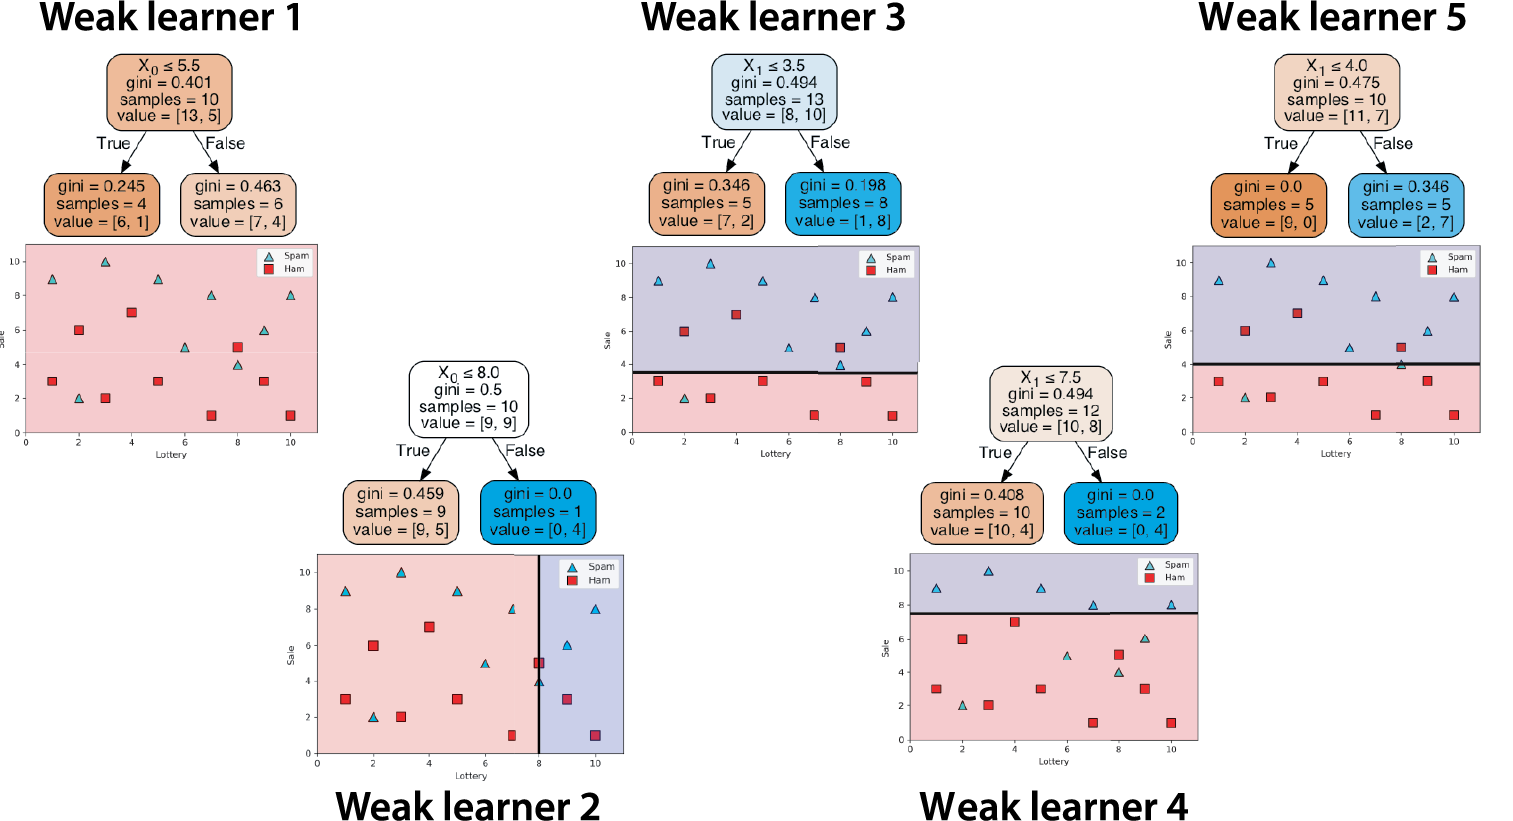
\includegraphics[width=\linewidth]{pic/decisionstumps.png}
        {\scriptsize Adopted from [4]}
    \end{figure}
    \endminipage
\end{frame}

\section{AdaBoost}

\subsection{Basic idea \& algorithm}

\begin{frame}{Basic idea}
    \begin{itemize}
        \itemsep1em
        \justifying
        \item \textbf{Sequential} production of classifiers
        \begin{itemize}
            \item Iteratively add the classifier whose addition will be most helpful.
        \end{itemize}
        \item Represent the important of each sample by assigning \textbf{weights} to them.
        \begin{itemize}
            \itemsep0.25em
            \item Correct classification $\implies$ smaller weights
            \item Misclassified samples $\implies$ larger weights
        \end{itemize}
        \item Each classifier is \textbf{dependent} on the previous ones.
        \begin{itemize}
            \item Focuses on the \textbf{previous ones’ error}.
        \end{itemize}
    \end{itemize}
\end{frame}

\begin{frame}{Example}
    \begin{center}
        \minipage{0.9\textwidth}
        \begin{figure}
            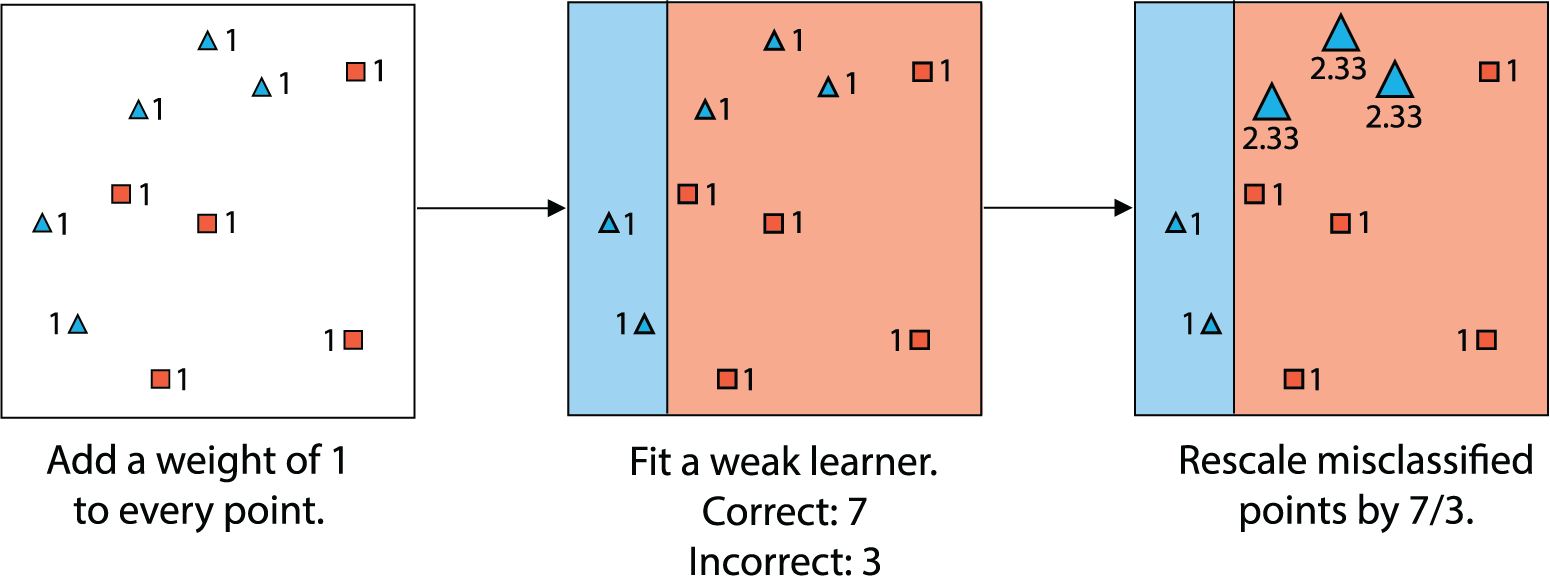
\includegraphics[width=\linewidth]{pic/adaboost_e1.png}
            {\scriptsize Adopted from [4]}
        \end{figure}
        \endminipage
    \end{center}
\end{frame}

\begin{frame}{Example, Cont.}
    \begin{center}
        \minipage{0.9\textwidth}
        \begin{figure}
            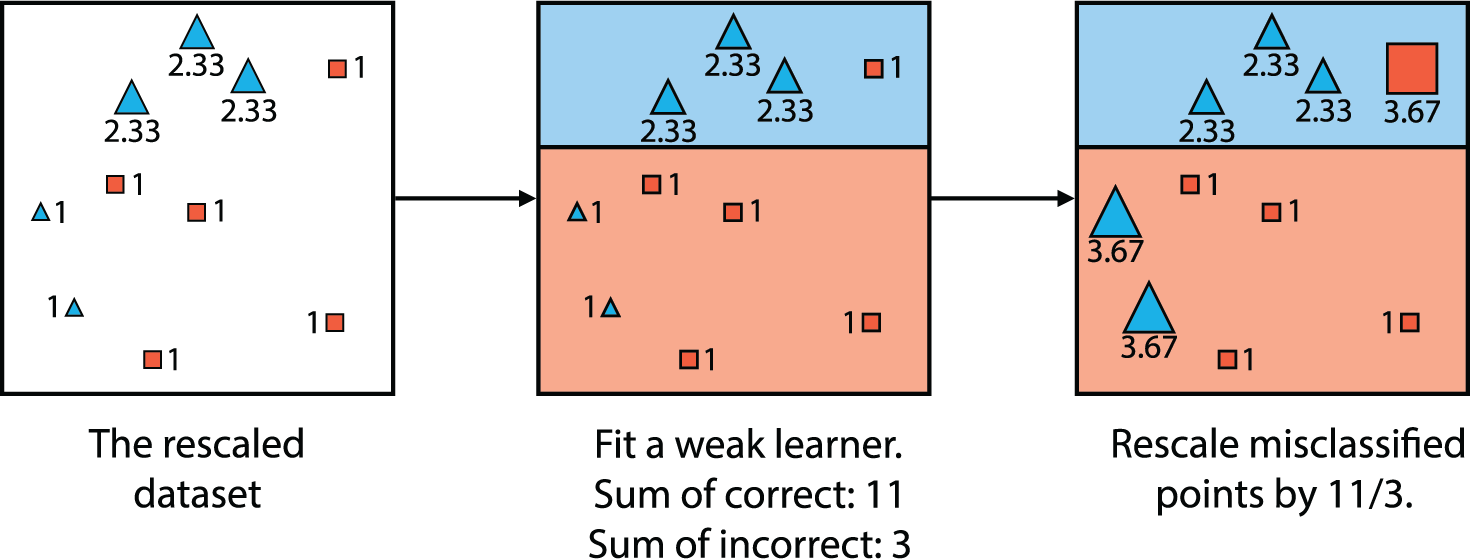
\includegraphics[width=\linewidth]{pic/adaboost_e2.png}
            {\scriptsize Adopted from [4]}
        \end{figure}
        \endminipage
    \end{center}
\end{frame}

\begin{frame}{Example, Cont.}
    \begin{center}
        \minipage{0.6\textwidth}
        \begin{figure}
            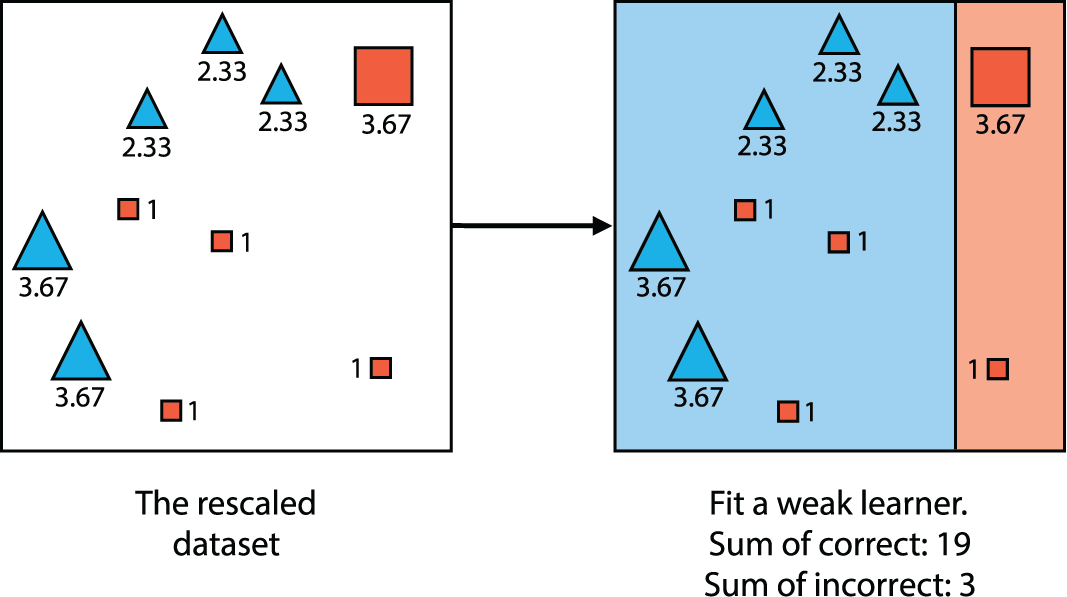
\includegraphics[width=\linewidth]{pic/adaboost_e3.png}
            {\scriptsize Adopted from [4]}
        \end{figure}
        \endminipage
    \end{center}
\end{frame}

\begin{frame}{Example, Cont.}
    \begin{center}
        \minipage{0.55\textwidth}
        \begin{figure}
            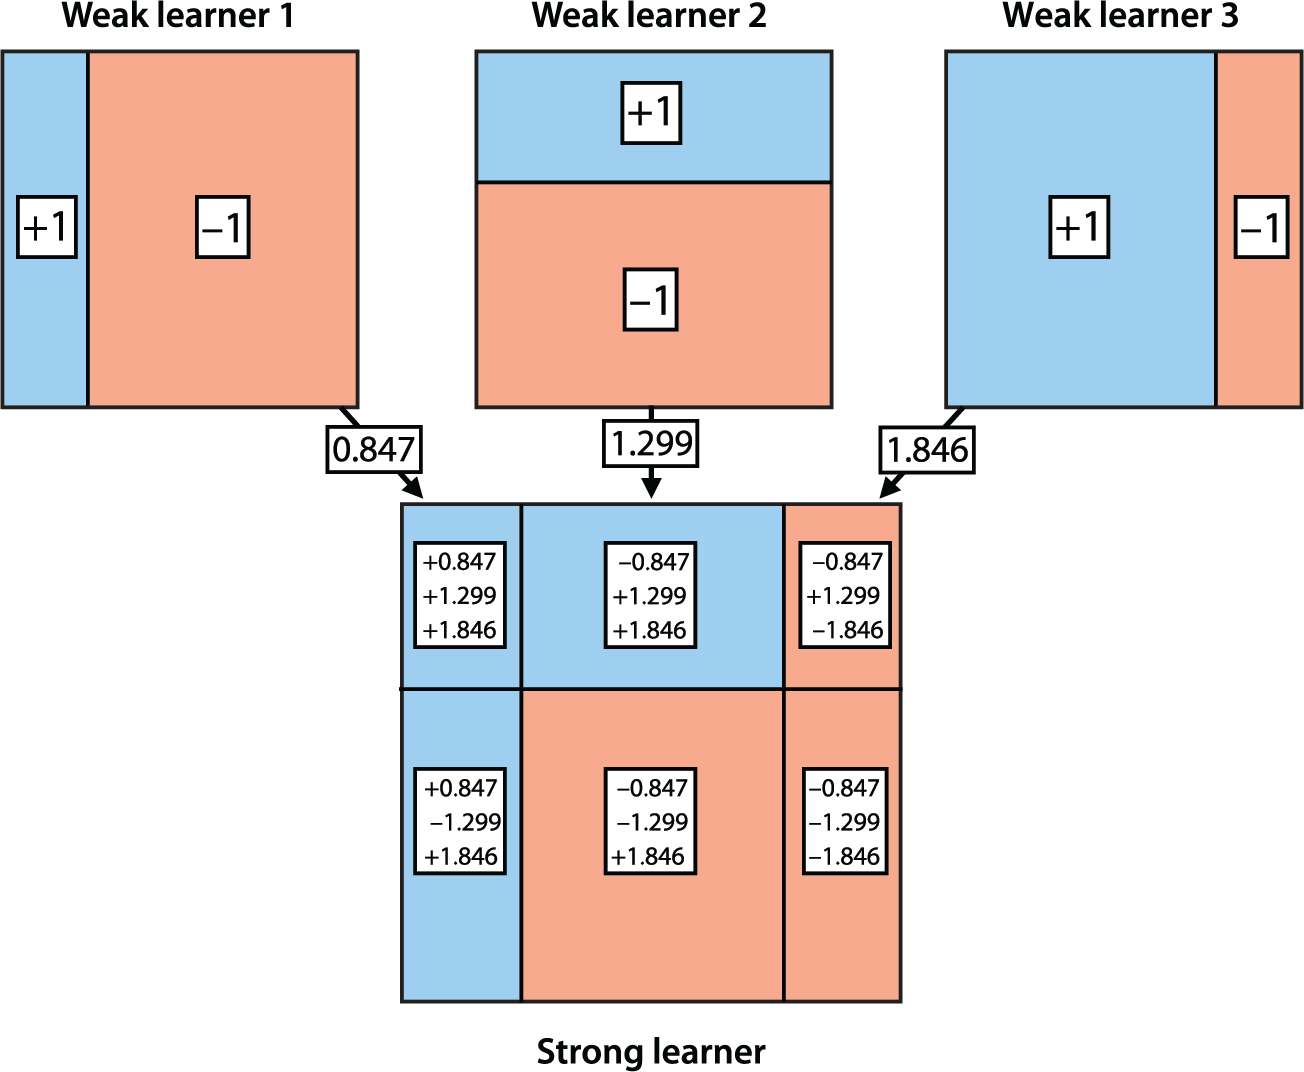
\includegraphics[width=\linewidth]{pic/adaboost_e4.png}
            {\scriptsize Adopted from [4]}
        \end{figure}
        \endminipage
    \end{center}
\end{frame}

\begin{frame}{Example, Cont.}
    \begin{center}
        \minipage{0.65\textwidth}
        \begin{figure}
            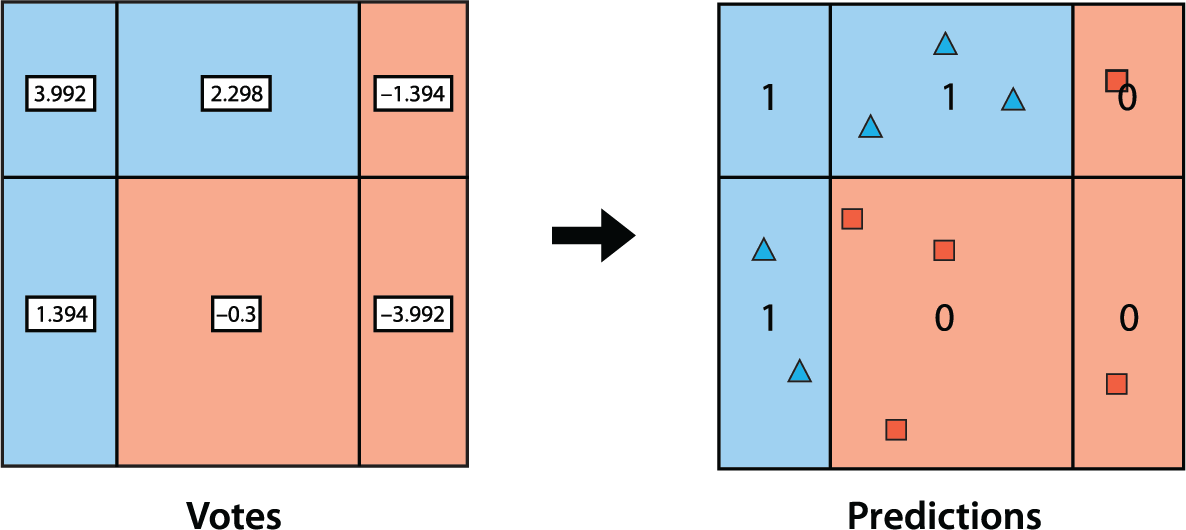
\includegraphics[width=\linewidth]{pic/adaboost_e5.png}
            {\scriptsize Adopted from [4]}
        \end{figure}
        \endminipage
    \end{center}
\end{frame}

\begin{frame}{Algorithm}
    \begin{itemize}
        \itemsep1em
        \justifying
        \item $H_M(\boldsymbol{x}) = \dfrac{1}{2}[\alpha_1h_1(\boldsymbol{x})+\dots+\alpha_Mh_M(\boldsymbol{x})] \longrightarrow$ the complete model \hfill $y^{(i)} \in \{-1, 1\}$
        \smallskip
        \begin{itemize}
            \itemsep0.5em
            \item $h_m(\boldsymbol{x})$: $m$-th weak learner
            \item $\alpha_m = \ \textcolor{deepred}{?} \longrightarrow$ votes of the $m$-th weak learner
        \end{itemize}
        \item $w_m^{(i)}$: weight of sample $i$ in iteration $m$
        \smallskip
        \begin{itemize}
            \item $w_{m+1}^{(i)} = \ \textcolor{deepred}{?}$
        \end{itemize}
        \item $J_m = \displaystyle\sum_{i=1}^N w_m^{(i)} \times I(y^{(i)} \neq h_m(\boldsymbol{x}^{(i)})) \longrightarrow$ loss of the $m$-th weak learner
        \item $\epsilon_m = \dfrac{\sum_{i=1}^N w_m^{(i)} \times I(y^{(i)} \neq h_m(\boldsymbol{x}^{(i)}))}{\sum_{i=1}^N w_m^{(i)}} \longrightarrow$ weighted error of the $m$-th weak learner
    \end{itemize}
\end{frame}

\begin{frame}{Algorithm, Cont.}
    \begin{itemize}
        \itemsep1em
        \justifying
        \item $H_M(\boldsymbol{x}) = \dfrac{1}{2}[\alpha_1h_1(\boldsymbol{x})+\dots+\alpha_Mh_M(\boldsymbol{x})] \longrightarrow$ the complete model \hfill $y^{(i)} \in \{-1, 1\}$
        \smallskip
        \begin{itemize}
            \itemsep0.5em
            \item $h_m(\boldsymbol{x})$: $m$-th weak learner
            \item $\alpha_m = \textcolor{deepred}{\ln\left(\dfrac{1 - \epsilon_m}{\epsilon_m}\right)} \longrightarrow$ votes of the $m$-th weak learner
        \end{itemize}
        \item $w_m^{(i)}$: weight of sample $i$ in iteration $m$
        \smallskip
        \begin{itemize}
            \item $w_{m+1}^{(i)} = \textcolor{deepred}{w_m^{(i)} e^{\alpha_m I(y^{(i)} \neq h_m(\boldsymbol{x}^{(i)}))}}$
        \end{itemize}
        \item $J_m = \displaystyle\sum_{i=1}^N w_m^{(i)} \times I(y^{(i)} \neq h_m(\boldsymbol{x}^{(i)})) \longrightarrow$ loss of the $m$-th weak learner
        \item $\epsilon_m = \dfrac{\sum_{i=1}^N w_m^{(i)} \times I(y^{(i)} \neq h_m(\boldsymbol{x}^{(i)}))}{\sum_{i=1}^N w_m^{(i)}} \longrightarrow$ weighted error of the $m$-th weak learner
    \end{itemize}
\end{frame}

\begin{frame}{Algorithm, Cont.}
    \begin{algorithm}[H]
    \caption{AdaBoost}\label{alg:AdaBoost}
    \begin{algorithmic}[1]
        \State Initialize data weight $w_1^{(i)} = \frac{1}{N}$ for all $N$ samples
        \For{$m=1$ to $M$}
            \State Find $h_m(\boldsymbol{x})$ by minimizing the loss: \hfill $J_m = \displaystyle\sum_{i=1}^N w_m^{(i)} \times I(y^{(i)} \neq h_m(\boldsymbol{x}^{(i)}))$
            \State Find the weighted error of $h_m(\boldsymbol{x})$: \hfill $\epsilon_m = \dfrac{\sum_{i=1}^N w_m^{(i)} \times I(y^{(i)} \neq h_m(\boldsymbol{x}^{(i)}))}{\sum_{i=1}^N w_m^{(i)}}$
            \State Assign votes $\alpha_m = \ln\left(\dfrac{1 - \epsilon_m}{\epsilon_m}\right)$
            \State Update the weights: \hfill $w_{m+1}^{(i)} = w_m^{(i)} e^{\alpha_m I(y^{(i)} \neq h_m(\boldsymbol{x}^{(i)}))}$
        \EndFor
        \State \textbf{Combined classifier:} $\hat{y} = \text{sign}(H_M(\boldsymbol{x}))$ where $H_M(\boldsymbol{x}) = \dfrac{1}{2}\sum_{m=1}^M \alpha_m h_m(\boldsymbol{x})$
    \end{algorithmic}
    \end{algorithm}
\end{frame}

% \begin{frame}{Notations \& conditions}
%     \begin{itemize}
%         \itemsep1em
%         \justifying
%         \item $w_m^{(i)}$: weighting coefficient of data point $i$ in iteration $m$
%         \item $\alpha_m$: weighting coefficient of $m$-th base classifier in the final ensemble
%         \item $\epsilon_m$: weighted error rate of $m$-th classifier 
%     \end{itemize}
%     \bigskip \bigskip
%     \begin{itemize}
%         \itemsep1em
%         \justifying
%         \item Only when $h_m(\boldsymbol{x})$ with $\epsilon_m < 0.5$ (better than chance) is found, boosting continues.
%         \begin{itemize}
%             \item Condorcet's jury theorem?
%         \end{itemize}
%     \end{itemize}
% \end{frame}

\subsection{Loss function \& proof}

\begin{frame}{Loss function}
    \begin{itemize}
        \itemsep1em
        \justifying
        \item There are many options for the loss function.
        \begin{itemize}
            \item AdaBoost is equivalent to using the following \textbf{exponential loss}.
        \end{itemize}
        \item[] \begin{center}
            $\mathcal{L}(y,H_M(\boldsymbol{x}))=e^{-y \times H_M(\boldsymbol{x})}$
        \end{center}
        \item[] \begin{center}
            $\hat{y}=\text{sign}(H_M(\boldsymbol{x}))$
        \end{center}
    \end{itemize}
\end{frame}

\begin{frame}{Why the exponential loss?}
    \minipage{0.54\textwidth}
    \begin{itemize}
        \itemsep1em
        \justifying
        \item Differentiable approximation (bound) of the $\boldsymbol{0/1}$ \textbf{loss}
        \begin{itemize}
            \itemsep0.25em
            \item Easy to optimize
            \item Optimizing an upper bound on classification error.
        \end{itemize}
    \end{itemize}
    \endminipage
    \hfill
    \minipage{0.39\textwidth}
    \begin{figure}
        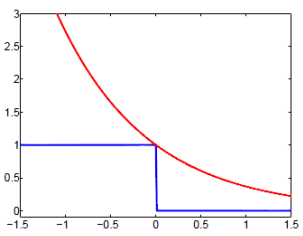
\includegraphics[width=\textwidth]{pic/exploss.png}
        {\scriptsize Adopted from [2]}
    \end{figure}
    \endminipage
\end{frame}

% \begin{frame}{Break down of the algorithm}
%     \begin{itemize}
%         \itemsep1em
%         \justifying
%         \item Now let's break down each step of the algorithm and show where they come from.
%         \begin{itemize}
%             \itemsep0.25em
%             \item \textbf{Step 1:} Calculate the exponential loss for the previous $H_M(\boldsymbol{x})$
%             \item \textbf{Step 2:} Derive the weighted error function, $J_m$
%             \item \textbf{Step 3:} Derive $\epsilon_m$ and $\alpha_m$
%             \item \textbf{Step 4:} Justify the weight update mechanism
%         \end{itemize}
%     \end{itemize}
% \end{frame}

\begin{frame}{Step 1: Calculating the exponential loss}
    \begin{itemize}
        \itemsep1em
        \justifying
        \item We need to calculate the exponential loss for:
        \item[] \begin{center}
            $H_m(\boldsymbol{x}) = 
            \text{\vertarrowbox[0ex]{\dfrac{1}{2}}{To have a cleaner form later}}
            [\alpha_1h_1(\boldsymbol{x})+\dots,+\alpha_mh_m(\boldsymbol{x})]$
        \end{center}
        \item \textbf{Idea:} consider adding the $m$-th component:
    \end{itemize}
    \begin{align*}
        \mathcal{L}_m &= \displaystyle\sum_{i=1}^N e^{-y^{(i)}H_m(\boldsymbol{x}^{(i)})} = \displaystyle\sum_{i=1}^N e^{-y^{(i)}[H_{m-1}(\boldsymbol{x}^{(i)}) + \frac{1}{2}\alpha_mh_m(\boldsymbol{x}^{(i)})]} \\
        &=\displaystyle\sum_{i=1}^N
        \text{\vertarrowbox[4ex]{e^{-y^{(i)}H_{m-1}(\boldsymbol{x}^{(i)})}}{Suppose it is fixed at stage $m$}}
        e^{-\frac{1}{2}\alpha_my^{(i)}h_m(\boldsymbol{x}^{(i)})}
        =\displaystyle\sum_{i=1}^N \underbrace{w_m^{(i)}}_{e^{-y^{(i)}H_{m-1}(\boldsymbol{x}^{(i)})}} 
        \text{\vertarrowbox[4ex]{e^{-\frac{1}{2}\alpha_my^{(i)}h_m(\boldsymbol{x}^{(i)})}}{Should be optimized at stage $m$ by seeking $h_m(\boldsymbol{x})$ and $\alpha_m$}}
    \end{align*}
\end{frame}

% \begin{frame}{Step 1: calculating the exponential loss, Cont.}
%     \begin{itemize}
%         \itemsep1em
%         \justifying
%         \item[] \begin{center}
%             $E=\displaystyle\sum_{i=1}^N w_m^{(i)} e^{-\frac{1}{2}\alpha_my^{(i)}h_m(\boldsymbol{x}^{(i)})}$
%         \end{center}
%         \item Sequentially adds a new component trained on reweighted training samples.
%         \item $w_m^{(i)}$: history of classification of $\boldsymbol{x}^{(i)}$ by $H_{m-1}$
%         \begin{itemize}
%             \item Loss weighted towards mistakes
%         \end{itemize}
%         \item Iteration $m$ optimization:
%         \begin{itemize}
%             \itemsep0.25em
%             \item Choose the new component, $h_m=h(\boldsymbol{x};\boldsymbol{\theta}_m)$
%             \item And the vote that optimizes the weighted exponential loss, $\alpha_m$.
%         \end{itemize}
%     \end{itemize}
% \end{frame}

\begin{frame}{Step 2: Deriving the weighted error function}
    \begin{itemize}
        \itemsep1em
        \justifying
        \item We need to derive the weighted error function, $J_m$
    \end{itemize}
    \begin{align*}
        \mathcal{L}_m &= \displaystyle\sum_{i=1}^N w_m^{(i)} e^{-\frac{1}{2}\alpha_my^{(i)}h_m(\boldsymbol{x}^{(i)})} \\
        &= e^{\frac{-\alpha_m}{2}} \left( \displaystyle\sum_{y^{(i)}=h_m(\boldsymbol{x}^{(i)})} w_m^{(i)} \right) + e^{\frac{\alpha_m}{2}} \left( \displaystyle\sum_{y^{(i)}\neq h_m(\boldsymbol{x}^{(i)})} w_m^{(i)} \right) \\
        &= (e^{\frac{\alpha_m}{2}}-e^{\frac{-\alpha_m}{2}}) \underbrace{\left(\displaystyle\sum_{y^{(i)}\neq h_m(\boldsymbol{x}^{(i)})} w_m^{(i)}\right)}_{\mathclap{J_m=\displaystyle\sum_{i=1}^Nw_m^{(i)} \times 
        \text{\vertarrowbox[2ex]{I}{\footnotesize Find $h_m(\boldsymbol{x})$ that minimizes $J_m$}}
        \left(y^{(i)} \neq h_m(\boldsymbol{x}^{(i)})\right)}} + e^{\frac{-\alpha_m}{2}} \left(\displaystyle\sum_{i=1}^Nw_m^{(i)}\right)
    \end{align*}
\end{frame}

\begin{frame}{Step 3: Deriving $\epsilon_m$ and $\alpha_m$}
    \begin{itemize}
        \itemsep1em
        \justifying
        \item We need to derive $\epsilon_m$ and $\alpha_m$ by setting the derivative equal to zero:
        \item[] \begin{center}
            $\dfrac{\partial \mathcal{L}_m}{\partial \alpha_m} = 0$
        \end{center}
        \item \textbf{Idea:} separate the derivative into misclassified and correctly classified samples.
    \end{itemize}
    \begin{align*}
        &\implies \frac{1}{2} (e^{\frac{\alpha_m}{2}} + e^{\frac{-\alpha_m}{2}}) \left(\displaystyle\sum_{y^{(i)}\neq h_m(\boldsymbol{x}^{(i)})} w_m^{(i)} \right) = \frac{1}{2}e^{\frac{-\alpha_m}{2}} \left(\displaystyle\sum_{i=1}^Nw_m^{(i)} \right) \\
        &\implies \dfrac{e^{\frac{-\alpha_m}{2}}}{(e^{\frac{\alpha_m}{2}} + e^{\frac{-\alpha_m}{2}})} = \dfrac{\sum_{y^{(i)}\neq h_m(\boldsymbol{x}^{(i)})} w_m^{(i)}}{\sum_{i=1}^Nw_m^{(i)}}
    \end{align*}
    \begin{itemize}
        \itemsep1em
        \justifying
        \item Set $\epsilon_m = \dfrac{\sum_{i=1}^N w_m^{(i)}I\left(y^{(i)} \neq h_m(\boldsymbol{x}^{(i)})\right)}{\sum_{i=1}^N w_m^{(i)}} \Longrightarrow \alpha_m = \ln\left(\dfrac{1 - \epsilon_m}{\epsilon_m}\right)$
    \end{itemize}
\end{frame}

\begin{frame}{Step 4: Justifying the weight update mechanism}
    \begin{itemize}
        \itemsep1em
        \justifying
        \item We need to justify the weight update mechanism.
        \item \textbf{Idea:} we have $w_m^{(i)}$ from the first step as $w_{m+1}^{(i)} = e^{-y^{(i)}H_{M}(\boldsymbol{x}^{(i)})}$
    \end{itemize}
    \begin{align*}
        &\xRightarrow{\text{separate } h_m(\boldsymbol{x}^{(i)})}w_{m+1}^{(i)} = w_m^{(i)} e^{-\frac{1}{2}\alpha_my^{(i)}h_m(\boldsymbol{x}^{(i)})} \\
        &\xRightarrow{y^{(i)}h_m(\boldsymbol{x}^{(i)}) = 1 - 2I\left(y^{(i)} \neq h_m(\boldsymbol{x}^{(i)})\right)} w_{m+1}^{(i)} = w_m^{(i)}
        \text{\vertarrowbox[0ex]{\ e^{-\frac{1}{2}\alpha_m}\ }{Independent of $i$ and can be ignored}}
        e^{\alpha_mI\left(y^{(i)} \neq h_m(\boldsymbol{x}^{(i)})\right)} \\ \\
        &\implies w_{m+1}^{(i)} = w_m^{(i)}e^{\alpha_m I\left(y^{(i)} \neq h_m(\boldsymbol{x}^{(i)})\right)}
    \end{align*}
\end{frame}

% \subsection{Summary \& example}

% \begin{frame}{Summary}
%     \begin{algorithm}[H]
%     \caption{AdaBoost Summary}\label{alg:AdaBoostSummary}
%     \begin{algorithmic}[1]
%     \For{$i = 1$ to $N$}
%         \State Initialize the data weight $w_1^{(i)} = \frac{1}{N}$
%     \EndFor
%     \For{$m = 1$ to $M$}
%         \State Find a classifier $h_m(\boldsymbol{x})$ by minimizing the weighted error function, $J_m$
%         \State Find the normalized weighted error of $h_m(\boldsymbol{x})$ as $\epsilon_m$
%         \State Compute the new component weight (share of votes) as $\alpha_m$
%         \State Update example weights for the next iteration $w_{m+1}^{(i)}$
%     \EndFor
%     \State Combined classifier $\hat{y}=\text{sign}(H_M(\boldsymbol{x}))$ where $H_M(\boldsymbol{x}) = \sum_{m=1}^M \alpha_m h_m(\boldsymbol{x})$
%     \end{algorithmic}
%     \end{algorithm}
% \end{frame}

% \begin{frame}{Example}
%     \begin{center}
%         \minipage{0.8\textwidth}
%         \begin{figure}
%             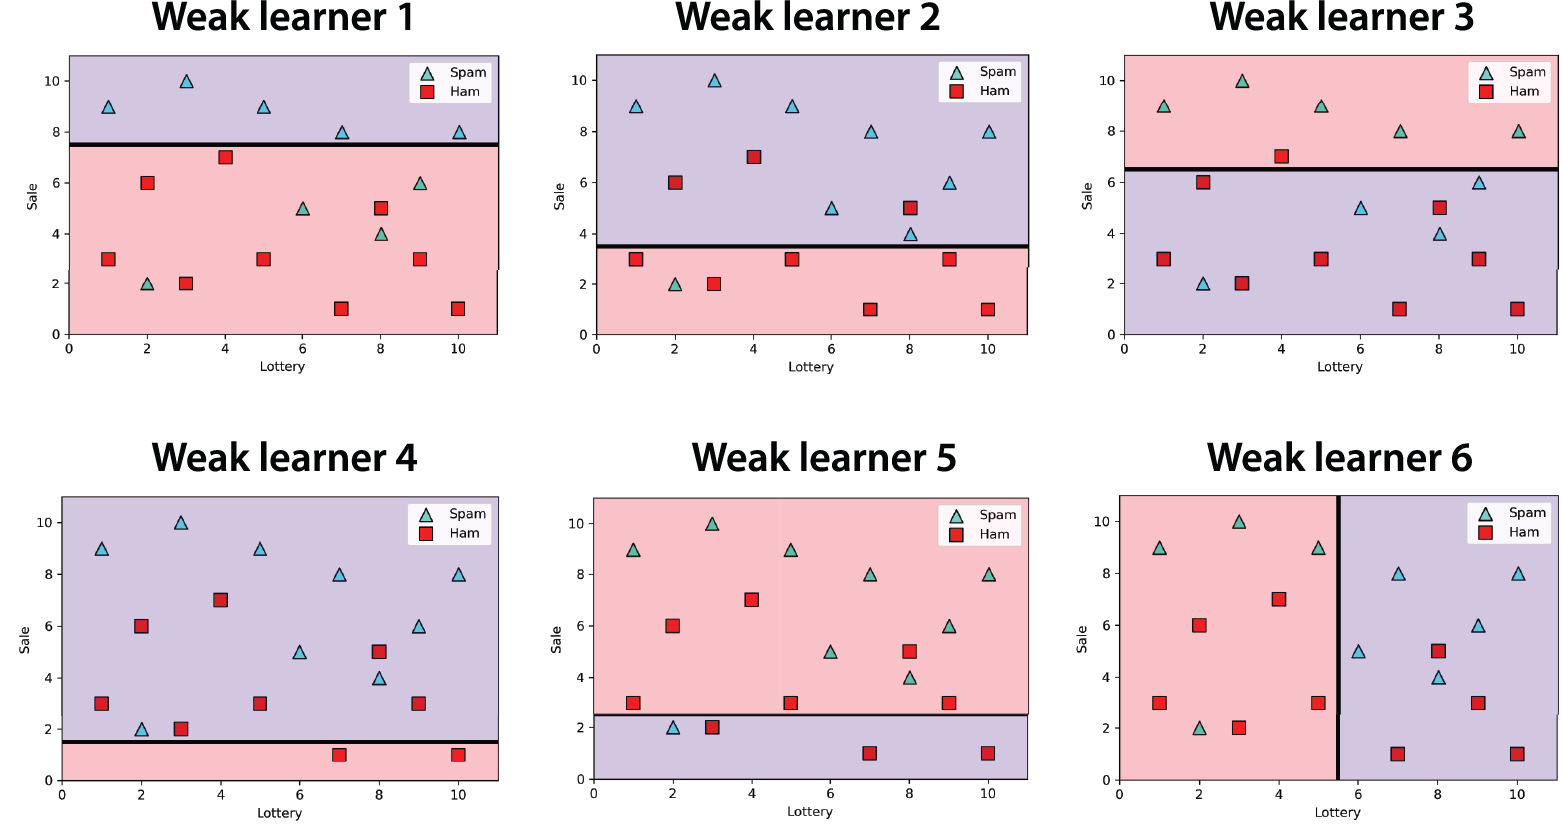
\includegraphics[width=\linewidth]{pic/adaboost_e11.png}
%             {\scriptsize Adopted from [4]}
%         \end{figure}
%         \endminipage
%     \end{center}
% \end{frame}

% \begin{frame}{Example, Cont.}
%     \begin{center}
%         \minipage{0.6\textwidth}
%         \begin{figure}
%             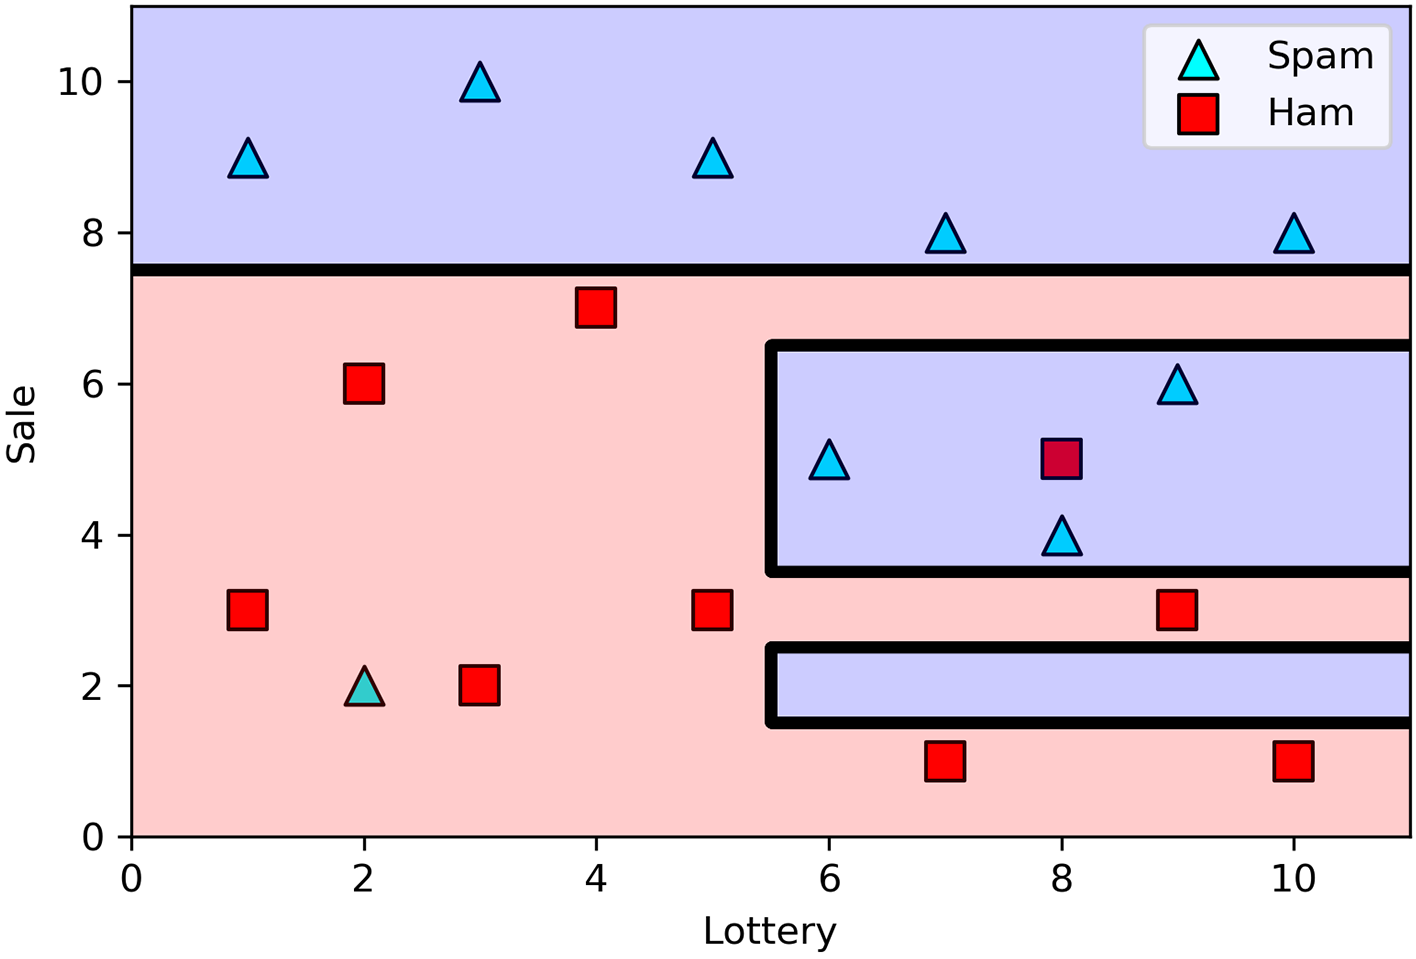
\includegraphics[width=\linewidth]{pic/adaboost_e12.png}
%             {\scriptsize Adopted from [4]}
%         \end{figure}
%         \endminipage
%     \end{center}
% \end{frame}

\subsection{Properties (extra-reading)}

\begin{frame}{Exponential loss properties}
    \begin{itemize}
        \itemsep1em
        \justifying
        \item In each boosting iteration, assuming we can find $h(\boldsymbol{x};\boldsymbol{\theta}_m)$ whose weighted error is better than chance.
        \item[] \begin{center}
            $H_m(x) = \frac{1}{2}[\alpha_1h(\boldsymbol{x};\boldsymbol{\theta}_1)+ \dots + \alpha_mh(\boldsymbol{x};\boldsymbol{\theta}_m)]$
        \end{center}
        \item Thus, \textbf{lower exponential loss} over training data is guaranteed.
    \end{itemize}
    \vfill
    \begin{center}
        \minipage{0.32\textwidth}
        \begin{figure}
            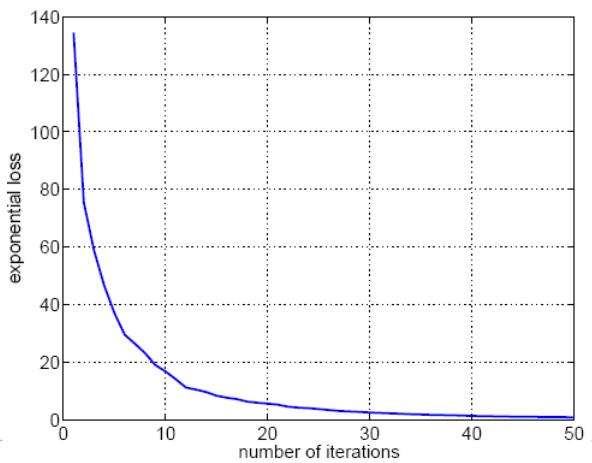
\includegraphics[width=\textwidth]{pic/boosting_exploss.png}
            {\scriptsize Adopted from [6]}
        \end{figure}
        \endminipage
    \end{center}
\end{frame}

\begin{frame}{Training error properties}
    \begin{itemize}
        \itemsep1em
        \justifying
        \item Boosting iterations typically \textbf{decrease} the \textbf{training error} of $H_M(\boldsymbol{x})$ over training examples.
    \end{itemize}
    \vfill
    \begin{center}
        \minipage{0.35\textwidth}
        \begin{figure}
            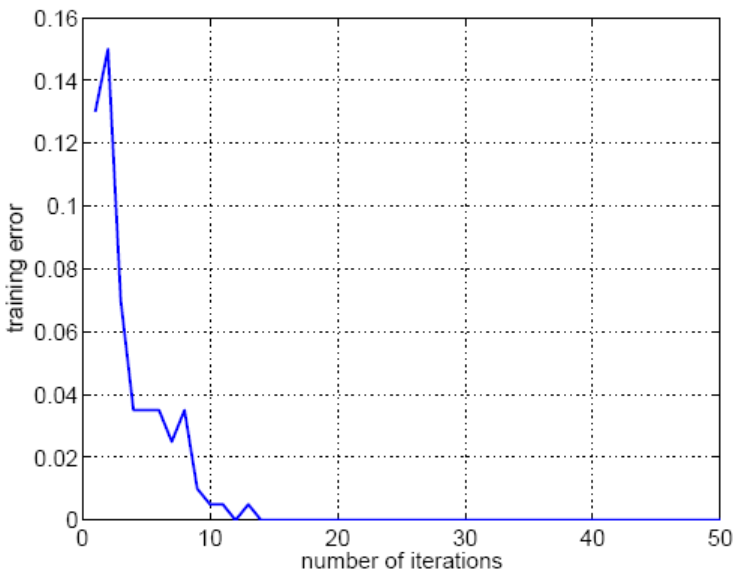
\includegraphics[width=\textwidth]{pic/boosting_train.png}
            {\scriptsize Adopted from [6]}
        \end{figure}
        \endminipage
    \end{center}
\end{frame}

\begin{frame}{Training error properties, Cont.}
    \begin{itemize}
        \itemsep1em
        \justifying
        \item \textbf{Training error} has to go \textbf{down exponentially fast} if the weighted error of each $h_m$ is strictly better than chance (i.e., $\epsilon_m < 0.5$)
        \item[] \begin{center}
            $E_{\text{train}}(H_M) \leq \displaystyle\prod_{m=1}^M 2\sqrt{\epsilon_m (1 - \epsilon_m)}$
        \end{center}
    \end{itemize}
    \vfill
    \begin{center}
        \minipage{0.35\textwidth}
        \begin{figure}
            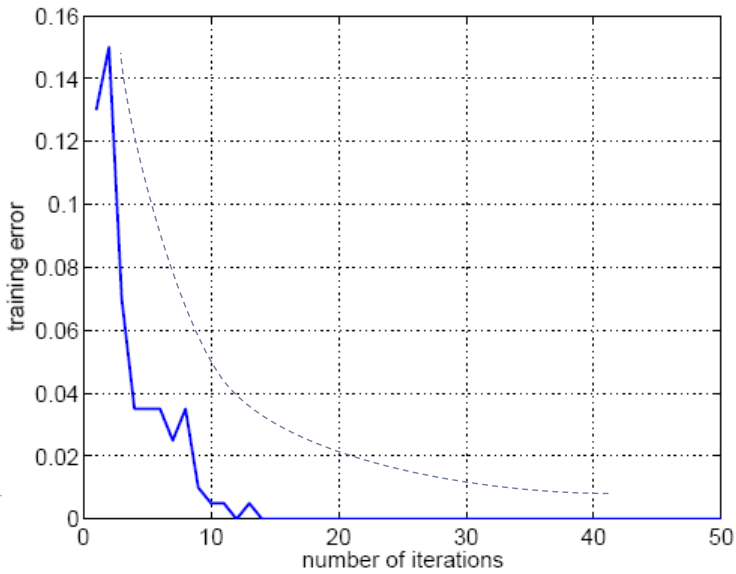
\includegraphics[width=\textwidth]{pic/boosting_trainexp.png}
            {\scriptsize Adopted from [6]}
        \end{figure}
        \endminipage
    \end{center}
\end{frame}

\begin{frame}{Weighted error properties}
    \begin{itemize}
        \itemsep1em
        \justifying
        \item \textbf{Weighted error} of each new component classifier tends to \textbf{increase} as a function of boosting iterations.
        \item[] \begin{center}
            $\epsilon_m = \dfrac{\sum_{i=1}^N w_m^{(i)}I\left(y^{(i)} \neq h_m(\boldsymbol{x}^{(i)})\right)}{\sum_{i=1}^N w_m^{(i)}}$
        \end{center}
    \end{itemize}
    \vfill
    \begin{center}
        \minipage{0.35\textwidth}
        \begin{figure}
            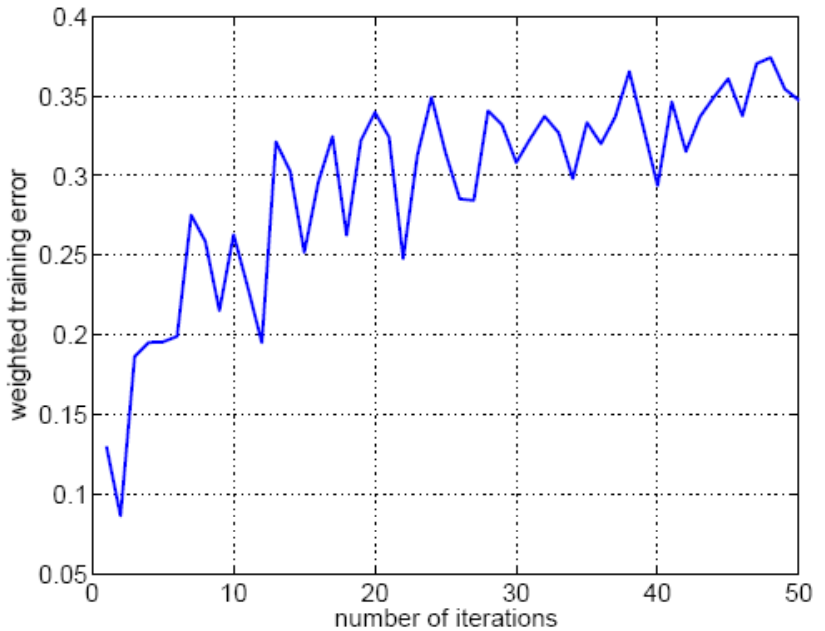
\includegraphics[width=\textwidth]{pic/boosting_weights.png}
            {\scriptsize Adopted from [6]}
        \end{figure}
        \endminipage
    \end{center}
\end{frame}

\begin{frame}{Test error properties}
    \begin{itemize}
        \itemsep1em
        \justifying
        \item \textbf{Test error} can still \textbf{decrease} after training error is flat (even zero).
        \item But, is it robust to overfitting?
        \begin{itemize}
            \item May easily overfit in the presence of labeling noise or overlap of classes.
        \end{itemize}
    \end{itemize}
    \vfill
    \begin{center}
        \begin{figure}[!htb]
        \minipage{0.35\textwidth}
            \centering
            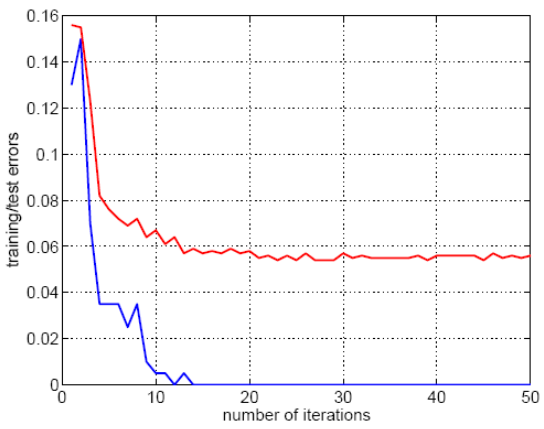
\includegraphics[width=\linewidth]{pic/boosting_traintest1.png}
            {\scriptsize Adopted from [6]}
        \endminipage \qquad
        \minipage{0.35\textwidth}
            \centering
            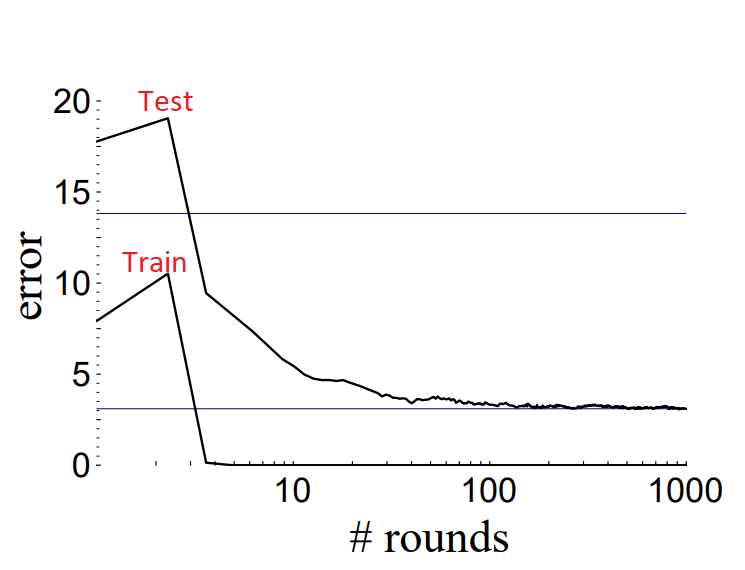
\includegraphics[width=\linewidth]{pic/boosting_traintest2.png}
            {\scriptsize Adopted from [3]}
        \endminipage
        \end{figure}
    \end{center}
\end{frame}

\begin{frame}{Typical behavior}
    \begin{itemize}
        \itemsep1em
        \justifying
        \item \textbf{Exponential loss} goes \textbf{strictly down}.
        \item \textbf{Training error} of $H$ goes \textbf{down}.
        \item Weighted error $\boldsymbol{\epsilon_m}$ goes \textbf{up} $\implies$ share of votes $\boldsymbol{\alpha_m}$ goes \textbf{down}.
        \item \textbf{Test error} \textbf{decreases} even after a flat training error.
    \end{itemize}
\end{frame}

\section{Comparison}

\begin{frame}{Bagging vs. Boosting}
    \begin{table}
    \centering
    \begin{tblr}{
      column{2} = {c},
      column{3} = {c},
      cells = {m, font=\footnotesize},
      cell{1}{2} = {silver},
      cell{1}{3} = {silver},
      cell{2}{1} = {silver},
      cell{3}{1} = {silver},
      cell{4}{1} = {silver},
      cell{5}{1} = {silver},
      cell{6}{1} = {silver},
      cell{7}{1} = {silver},
      vline{2-4} = {1}{},
      vline{-} = {2-7}{},
      hline{1} = {2-3}{},
      hline{2-8} = {-}{},
    }
                                 & \textbf{Bagging}                     & \textbf{Boosting}                             \\
    \textbf{Training Strategy}   & Parallel training                    & Sequential training                           \\
    \textbf{Data Sampling}       & {Bootstrapping\\(random subsets)}    & {Weighted \\(by instance importance)}         \\
    \textbf{Learners Dependency} & Independent                          & {Dependent\\(on the previous models)}         \\
    \textbf{Learner Weighting}   & Equal weights                        & {Varying weights\\(based on importance)}      \\
    \textbf{Tolerance to Noise}  & {More robust \\(due to aggregation)} & {More sensitive \\(may overfit to noise)}     \\
    \textbf{Properties}          & Reduces variance                     & {Reduces bias and variance \\(focus on bias)} 
    \end{tblr}
    \end{table}
\end{frame}

\section{References}

\begin{frame}{Contributions}
    \begin{itemize}
    \itemsep1em
    \justifying
        \item \textbf{This slide has been prepared thanks to:}
    \begin{itemize}
        \itemsep1em
        \item \href{https://github.com/NikanV/}{Nikan Vasei}
        \item \href{https://github.com/Mahan-Bayhaghi}{Mahan Bayhaghi}
    \end{itemize}
    \end{itemize}
\end{frame}

\begin{frame}[allowframebreaks]
    \bibliography{ref}
    \bibliographystyle{ieeetr}
    \nocite{*}
\end{frame}

\end{document}
